\documentclass[12pt,a4paper]{article}

% === Packages ===
\usepackage[utf8]{inputenc}
\usepackage[T1]{fontenc}
\usepackage{amsmath,amssymb,amsthm}
\usepackage{bm}
\usepackage[margin=1in]{geometry}
\usepackage{graphicx}
\usepackage[round,authoryear]{natbib}
\usepackage{booktabs}
\usepackage{url}   % long URLs in the code-availability statement need breakable links
\usepackage{multirow}
\usepackage{algorithm}
\usepackage{algpseudocode}
\usepackage{xcolor}
\usepackage{setspace}
\usepackage{placeins}
\usepackage{indentfirst}   % indent the first paragraph after every heading as well
% Single-spaced for submission; the journal's own class is applied at acceptance.
% Allow TeX a slightly looser third pass so that long unbreakable items (URLs, inline
% formulas) are set without protruding into the margin.
\setlength{\emergencystretch}{1em}

% === Theorem environments ===
\newtheorem{theorem}{Theorem}[section]
\newtheorem{lemma}[theorem]{Lemma}
\newtheorem{proposition}[theorem]{Proposition}
\newtheorem{corollary}[theorem]{Corollary}
\newtheorem{assumption}{Assumption}[section]
\theoremstyle{definition}
\newtheorem{definition}[theorem]{Definition}
\theoremstyle{remark}
\newtheorem{remark}[theorem]{Remark}

% === Notation ===
\newcommand{\R}{\mathbb{R}}
\newcommand{\E}{\mathbb{E}}
\newcommand{\Pbb}{\mathbb{P}}
\newcommand{\cN}{\mathcal{N}}
\newcommand{\cC}{\mathcal{C}}
\newcommand{\cS}{\mathcal{S}}
\newcommand{\ind}[1]{\mathbf{1}\{#1\}}
\newcommand{\norm}[1]{\|#1\|}
\newcommand{\abs}[1]{|#1|}
\newcommand{\supp}{\mathrm{supp}}
\newcommand{\argmin}{\mathop{\mathrm{argmin}}}
\newcommand{\rht}{\tilde{\rho}_\tau}
\newcommand{\psit}{\psi_\tau}
\newcommand{\betah}{\hat{\beta}}
\newcommand{\betas}{\beta^*}
\newcommand{\sigmah}{\hat{\sigma}}
\newcommand{\bbar}{\bar{\beta}}
\newcommand{\muv}{\mu_W}
\newcommand{\Sxw}{\Sigma_{x|w}}
\newcommand{\Ccal}{C}

\begin{document}

\title{The Smoothed-Check-Loss Trap: \\ Why Convolution-Based Corrections Fail \\ in
Quantile Regression with Measurement Error}

\author{Kaixu Cai \\[2pt]
\parbox{0.82\textwidth}{\centering\itshape School of Mathematics and Statistics,
Guangxi Normal University, Guilin 541006, China} \\[2pt]
\texttt{1006282498@qq.com}}

\date{}

\maketitle

\begin{abstract}
Quantile regression with covariate measurement error is well understood in fixed
dimension, where corrected scores \citep{stefanski1989,nakamura1990,wang2012correctedloss}
and conditional estimating equations \citep{wei2009quantile} give consistent estimators,
and penalised high-dimensional versions of these routes exist
\citep{kaul2015weighted,bai2021variable,ma2022highdim}. What is missing is a theory for the
shortcut used in practice and for calibration-based inference when the covariates outnumber
the observations, and that is what this paper provides. We study
the two natural routes. The first, replacing the check loss by its convolution with the
measurement error distribution, is closed-form and convex but not a correction: writing
$\Sigma_u$ for the measurement-error covariance, $\betas$ for the true coefficient vector
and $M\succeq0$ for the kernel covariance, we show that the population score at the truth
equals $(\Sigma_u+M)\betas\,d_M$ for a positive scalar $d_M$ depending on the kernel and
the error density. This holds for \emph{every} kernel, including the self-consistent choice
$M=\Sigma_u$, for which the gradient is exactly twice the fixed-scale one. The target therefore moves by
$\Theta(\norm{\Sigma_u\betas})$ and never returns, and the smoothed estimator shares that
target with the naive one, exactly so under the Gaussian design. The second route works: conditioning gives
$\muv=\E[X\mid W]$, under which $Y=\muv^\top\betas+e$ with $e$ independent of $\muv$, so
quantile regression of $Y$ on $(\muv,1)$ is correctly specified and its score is exactly
mean-zero. We give $\ell_1$ oracle inequalities in $p\gg n$, first for a known and then for
an \emph{estimated} calibration, where a perturbation lemma, a sup-norm score bound and a
restricted-eigenvalue transfer are required. Debiased intervals are then constructed, and we
prove their asymptotic normality with the oracle-calibration variance under an explicit
condition on the calibration: the design-error part of the penalty must be $o_P(n^{-1/2})$.
A known calibration satisfies it, while the sample-covariance plug-in does not, its row-wise
error being of order $\sqrt{\log p/n}$, and we give the resulting bias and its coverage cost.
An application to NHANES, where the measurement error covariance is
estimated from two dietary recalls rather than assumed, shows the correction changing
coefficient magnitudes severalfold.
\end{abstract}

\noindent\textbf{Keywords:} Measurement error; quantile regression; regression
calibration; corrected score; smoothed check loss; errors-in-variables; debiased inference.

\medskip
\noindent\textbf{MSC 2020 subject classifications.} Primary 62J05; secondary 62G08, 62G20,
62J07, 62H12.

\medskip
\noindent\textbf{Running title.} The smoothed-check-loss trap.

% ============================================================
\section{Introduction}
% ============================================================

Covariates are rarely observed exactly: RNA-seq expression is noisy
\citep{carroll2006measurement}, pollutant exposures are interpolated from sparse monitors
\citep{gryparis2009measurement}, imaging connectivity has test--retest reliability far below
one \citep{noble2017}, and dietary intake from 24-hour recall, our example in
\S\ref{sec:nhanes}. Classical measurement error $W=X+U$ attenuates mean-regression
coefficients, and quantile regression \citep{koenker1978} describes effects away from the
centre.

For mean regression the remedies are standard: correct the loss, the score, or the design
\citep{fuller1987,carroll2006measurement}. The most portable is the \emph{corrected score} of
\citet{stefanski1989} and \citet{nakamura1990}, needing only the measurement error
distribution but a polynomial--exponential loss. The check loss
$\rho_\tau(u)=u(\tau-\ind{u<0})$ is not of that type; the recipe used instead
\emph{convolves the loss} with the measurement error distribution, as
$U^\top\beta\sim\cN(0,\beta^\top\Sigma_u\beta)$, giving the closed form
\begin{equation}
\rht(r,\sigma) \;=\; r\Big[\Phi\!\Big(\frac{r}{\sigma}\Big)-(1-\tau)\Big]
+ \sigma\phi\!\Big(\frac{r}{\sigma}\Big),
\qquad \sigma^2 = \beta^\top\Sigma_u\beta,
\label{eq:loss}
\end{equation}
with $\Phi,\phi$ the standard normal cdf and density, and smoothed score
$\psit(r,\sigma)=\Phi(r/\sigma)-(1-\tau)$.

This article is about what \eqref{eq:loss} estimates. It is the check loss convolved
with $\cN(0,\sigma^2)$,
\begin{equation}
\rht(r,\sigma) = \E_{Z\sim\cN(0,\sigma^2)}\big[\rho_\tau(r-Z)\big],
\label{eq:identity}
\end{equation}
so minimising the empirical $\rht(Y-W^\top\beta,\sigma)$ adds $Z$ to a residual that already
contains $U^\top\beta$: two independent copies of the measurement error along $\beta$.

\paragraph{Smoothing cannot work (Theorem~\ref{thm:score}, Lemma~\ref{lem:bias},
Proposition~\ref{prop:target}).} The population score is
$\E[W\psit(r_i^*,\sigma)]=-(\Sigma_u\betas)\,d(\sigma)$, with
$d(\sigma)=(\cN(0,\sigma^{*2}+\sigma^2)*f_\varepsilon)(0)>0$ and
$\sigma^{*2}={\betas}^\top\Sigma_u\betas$: the bias is of order $\|\Sigma_u\betas\|$, does not
vanish with $n$, and cannot be tuned away, the identity holding for all $\sigma>0$. A
first-order expansion, exact under the Gaussian design
(Proposition~\ref{prop:exact-target}), identifies the target as the \emph{attenuated}
parameter $\bbar=(\Sigma_x+\Sigma_u)^{-1}\Sigma_x\betas$,
$\|\bbar-\betas\|\ge\|\Sigma_u\betas\|\,d(\sigma)\,\sigma/(\lambda_{\max}(\Sigma_x+\Sigma_u)\phi(0))$,
also the target of \emph{naive} quantile regression on $W$
(Corollary~\ref{cor:same-target}), bounded away from zero by the mean value theorem. No
other convolution repairs it (Corollary~\ref{cor:no-conv}): any kernel covariance
$\Sigma_k\succ0$ leaves $\E[W\psit]=-(\Sigma_k\betas)\,d_k$ non-zero whenever
$\Sigma_k\betas\neq0$, so the \emph{posterior} covariance of $X$ given $W$ is still
inconsistent, its self-consistent scale minimising at the attenuated value
(Proposition~\ref{prop:posterior-adaptive}, verified in \S\ref{sec:targets}).

\paragraph{The correct operation is conditioning (Theorem~\ref{thm:calib}).} Under a Gaussian
design the calibrated covariate $\muv=\Ccal W$, with
$\Ccal=\Sigma_x(\Sigma_x+\Sigma_u)^{-1}$, gives $Y=\muv^\top\betas+e$ with $e$ independent of
$\muv$ and $Q_\tau(e\mid\muv)=\delta_\tau$ constant, so quantile regression of $Y$ on
$(\muv,1)$ is correctly specified, with slope $\betas$ for all $\tau$. The calibrated score
is exactly mean-zero, so the debiasing of \S\ref{sec:debiasing} applies here but not to the
smoothed loss. Theorem~\ref{thm:lowdim} and Theorem~\ref{thm:highdim}
give the fixed-dimensional and $\ell_1$-oracle results.

\medskip
\noindent\textbf{Relation to the literature.}
Corrected scores go back to \citet{stefanski1989} and \citet{nakamura1990}, surveyed with the
wider field by \citet{fuller1987} and \citet{carroll2006measurement}. Three fixed-dimension
corrections work: orthogonal residuals under spherical symmetry \citep{he2000quantile}; the
unbiased conditional estimating equation
$n^{-1}\sum_i\int_x \Psi_\tau(y_i-x^\top\beta)x\,f(x\mid y_i,w_i)\,dx=0$, solved by
\citet{wei2009quantile} through EM over quantile levels; and a smoothed loss that
\citet{wang2012correctedloss} debias by \citet{stefanski1989}'s complex-argument device
(normal errors) or a second-derivative correction (Laplace errors). Our negative result in
\S\ref{sec:negative} concerns not these but the shortcut of convolving the check loss with the
measurement error distribution at a bandwidth fixed at the error scale
(Proposition~\ref{prop:exact-target}).

In high dimensions, \citet{kaul2015weighted} prove $\ell_1$ consistency for a weighted
corrected score with many covariates, targeting $\betas$ rather than the attenuated
parameter; \citet{bai2021variable} treat quantile regression with
missingness and measurement error through a corrected loss; \citet{ma2022highdim} a general
Lipschitz loss. Instrumental-variable identification goes to \citet{schennach2008quantile};
censored-data work uses smoothed and corrected scores \citep{ma2011censored,wu2015smoothed}
and SIMEX \citep{shang2012measurement,tekwe2022estimation}, the latter on NHANES
physical-activity data. None uses the raw design $W$ with fixed bandwidth.

For high-dimensional quantile regression without measurement error we rely on
\citet{belloni2011l1} and \citet{wang2012}, for regularised $M$-estimation on
\citet{negahban2012unified} and \citet{buhlmann2011statistics}, and for mean-regression
measurement error on \citet{rosenbaum2010}, \citet{datta2017cocolasso} and
\citet{loh2012highdim}; the smoothed check loss is the device of
\citet{fernandes2021smoothing} and \citet{he2023smoothed} at a vanishing bandwidth, and our
debiasing follows \citet{zhang2014confidence},
\citet{vandegeer2014asymptotically} and \citet{javanmard2014hypothesis}, with
\citet{bradic2017uniform} for quantile regression. Regression calibration
\citep{carroll2006measurement} is the device our estimator uses.

% ============================================================
\section{Setup and the smoothing identity}
\label{sec:setup}
% ============================================================

We observe $n$ independent copies $\{(Y_i,W_i)\}_{i=1}^n$ of
\begin{align}
Y_i &= X_i^\top\betas + \varepsilon_i, \qquad Q_\tau(\varepsilon_i\mid X_i) = 0,
\label{eq:model}\\
W_i &= X_i + U_i, \qquad U_i \sim \cN(0,\Sigma_u),
\label{eq:me}
\end{align}
with $X_i,\betas\in\R^p$, $Q_\tau$ the conditional $\tau$-quantile, and $\Sigma_u$ known.
When $\Sigma_u=\sigma_u^2I_p$ we write $\sigma_u$ for the scalar noise level, so that
$\rho=\sigma_u\norm{\betas}$ and $\sigma(\beta)=\sigma_u\norm{\beta}$; $\sigma_u$ is
reserved for that isotropic case, while $\sigma$ denotes a smoothing bandwidth throughout.
Write $\rho_\tau(u) = u(\tau-\ind{u<0})$ for the check loss,
$r_i^* = Y_i - W_i^\top\betas = \varepsilon_i - U_i^\top\betas$ for the residual at the
truth, and
\begin{equation}
\sigma^{*2} = {\betas}^\top\Sigma_u\betas,\qquad
\sigma^2(\beta) = \beta^\top\Sigma_u\beta ,
\qquad
\rho := \norm{\Sigma_u\betas} .
\label{eq:rho}
\end{equation}
Unless stated otherwise $\|\betas\|_0 = s \ll n \ll p$ and $X_i$ is sub-Gaussian with
$\E[X_i]=0$ and $\lambda_{\min}(\Sigma_x)\ge\kappa_x>0$; Gaussianity of $X$ is needed only
in \S\ref{sec:fix}, where the calibration identity is derived, and is stated there
(Assumption~\ref{ass:gauss}).

\begin{lemma}[The corrected loss is a smoothed check loss]
\label{lem:identity}
For every $r\in\R$ and $\sigma>0$ the right-hand side of \eqref{eq:loss} satisfies
\eqref{eq:identity}. Moreover
\begin{equation}
\frac{\partial}{\partial r}\rht(r,\sigma) = \psit(r,\sigma) = \Phi(r/\sigma)-(1-\tau),
\qquad
\frac{\partial^2}{\partial r^2}\rht(r,\sigma) = \frac{1}{\sigma}\phi(r/\sigma) > 0 ,
\end{equation}
so $\rht(\cdot,\sigma)$ is strictly convex, and $\rht(r,\sigma)\to\rho_\tau(r)$ as
$\sigma\downarrow0$.
\end{lemma}

\begin{proof}
See Appendix~\ref{app:proofs}.
\end{proof}

\begin{remark}[What smoothing buys, and what it contains]
\label{rem:double}
By Lemma~\ref{lem:identity}, the population objective of a fixed-scale smoothed
estimator is
\begin{equation}
L_\sigma(\beta) = \E\big[\rht(Y-W^\top\beta,\sigma)\big]
= \E\big[\rho_\tau\big(Y-X^\top\beta-U^\top\beta-Z\big)\big],
\qquad Z\sim\cN(0,\sigma^2),
\label{eq:double}
\end{equation}
with $Z$ independent of $(X,U,\varepsilon)$. At $\beta=\betas$ the argument of the check loss is
$\varepsilon_i - U_i^\top\betas - Z_i$, whose variance is
$\mathrm{Var}(\varepsilon)+\sigma^{*2}+\sigma^2$: the measurement error enters \emph{with}
the added Gaussian, not instead of it, and Section~\ref{sec:negative} shows that this is not
a cosmetic difference, because it moves the minimiser. For fixed $\sigma$ the objective
$\beta\mapsto L_\sigma(\beta)$ is convex, which is the practical advantage usually attributed
to \eqref{eq:loss}; Lemma~\ref{lem:identity} identifies the price, namely that the same
smoothing which convexifies the loss also changes the parameter it estimates. A convex
surrogate for computation must therefore be paired with a target corrected separately, which
is what \S\ref{sec:fix} does.
\end{remark}

% ============================================================
\section{The smoothed loss targets the attenuated parameter}
\label{sec:negative}
% ============================================================

Throughout, $\sigma>0$ is a \emph{fixed} scale, as in two-stage algorithms that hold a pilot
scale fixed. No sparsity or dimension condition is imposed.

\begin{theorem}[The smoothed score has a non-vanishing mean]
\label{thm:score}
Assume $X_i$ is independent of $(U_i,\varepsilon_i)$ with $\E[X_i]=0$, that
$U_i\sim\cN(0,\Sigma_u)$ is independent of $\varepsilon_i$, and that
$f_\varepsilon$, the density of $\varepsilon_i$, is bounded and continuous at $0$ with
$f_\varepsilon(0)>0$. Then for every fixed $\sigma>0$
\begin{equation}
\E\big[W_i\,\psit(r_i^*,\sigma)\big] = -\,\Sigma_u\betas \,\cdot\, d(\sigma),
\qquad
d(\sigma) := \big(\cN(0,\sigma^{*2}+\sigma^2)*f_\varepsilon\big)(0) > 0 .
\label{eq:score-bias}
\end{equation}
In particular the score is mean-zero at $\betas$ only if $\Sigma_u\betas = 0$, i.e.\ only
if the measurement error does not affect the regression function.
\end{theorem}

\begin{proof}
See Appendix~\ref{app:proofs}.
\end{proof}

\begin{remark}
The bias is $O(\|\Sigma_u\betas\|)$, independent of $n$, and non-zero at every $\sigma>0$:
no data-driven scale, including a pilot-based $\sigmah$, removes it.
\end{remark}

\begin{theorem}[No convolution kernel is a corrected score]
\label{thm:kernel-class}
Let $G$ be a distribution on $\R$ with a density $g$ that is continuous at $0$ with
$g(0)>0$, and define the convolved loss
$\rho_G(r) = \E_{V\sim G}[\rho_\tau(r-V)]$, its score
$\psi_G(r) = F_G(r)-(1-\tau)$ and $L_G(\beta) = \E[\rho_G(Y-W^\top\beta)]$. Under the
remaining assumptions of Theorem~\ref{thm:score},
\begin{equation}
\E\big[W_i\,\psi_G(r_i^*)\big] \;=\; -\,\Sigma_u\betas\,\cdot\,D_G,
\qquad
D_G := \E\big[g(\varepsilon_i-Z_i)\big] > 0,
\quad Z_i\sim\cN(0,\sigma^{*2}) ,
\label{eq:kernel-bias}
\end{equation}
and consequently $\nabla L_G(\betas) = \Sigma_u\betas\,D_G$. Gaussian $G=\cN(0,\sigma^2)$
recovers Theorem~\ref{thm:score} with $D_G = d(\sigma)$. Hence for \emph{any} kernel with
a positive density at zero, the smoothed loss is stationary at $\betas$ only if
$\Sigma_u\betas=0$, including kernels whose covariance is unrelated to $\Sigma_u$ and in
particular the posterior covariance $\Sxw$ suggested by calibration.
\end{theorem}

\begin{proof}
See Appendix~\ref{app:proofs}.
\end{proof}

\begin{theorem}[A scale that adapts to $\beta$ does not repair the bias either]
\label{thm:adaptive}
Fix any $M\succeq0$ with $M\betas\neq0$ and let
$L_{\mathrm{ad}}(\beta) = \E[\rht(Y-W^\top\beta,\sigma_M(\beta))]$ with
$\sigma_M(\beta)=\sqrt{\beta^\top M\beta}$; write $s_M=\sigma_M(\betas)$ and
$d_M = d(s_M) = (\cN(0,\sigma^{*2}+s_M^{2})*f_\varepsilon)(0)$. Under the assumptions of
Theorem~\ref{thm:score}, using $\partial\rht(r,\sigma)/\partial\sigma = \phi(r/\sigma)$ and
$\nabla\sigma_M(\beta) = M\beta/\sigma_M(\beta)$,
\begin{equation}
\nabla L_{\mathrm{ad}}(\betas)
= \underbrace{\Sigma_u\betas\,d_M}_{\text{fixed-scale part}}
\;+\;\underbrace{\E\Big[\phi\Big(\frac{r_i^*}{s_M}\Big)\Big]\frac{M\betas}{s_M}}
_{\text{scale-adaptation part}}
= \;\big(\Sigma_u+M\big)\betas\; d_M .
\label{eq:adaptive}
\end{equation}
Consequently $\betas$ is not stationary whenever $(\Sigma_u+M)\betas\neq0$, whatever the
kernel matrix $M$. Two choices of $M$ matter in practice. For the self-consistent scale
$M=\Sigma_u$ the gradient is $2\Sigma_u\betas d_{M}$, exactly \emph{twice} the
fixed-scale gradient of Theorem~\ref{thm:score}; the exact targets at $\sigma_u=0.5$ are
$1.600$ for the fixed-scale form and $1.333$ for this one, against $\betas=2$
(Table~S8 of Online Resource~1 and Proposition~\ref{prop:exact-target}). For the posterior
kernel $M=\Sxw$ the gradient is $(\Sigma_u+\Sxw)\betas\,d_M$, which is non-zero as well;
this is the control experiment of \S\ref{sec:targets}, and it shows that the natural
repair suggested by calibration, convolving with the smaller posterior covariance rather
than with $\Sigma_u$, fails for the same reason. If instead the smoothed loss is
evaluated at the calibrated regressor and the scale is made self-consistent, the
minimiser moves to $\bbar$ exactly; see Proposition~\ref{prop:posterior-adaptive}.
\end{theorem}

\begin{proof}
See Appendix~\ref{app:proofs}.
\end{proof}

\begin{remark}
The complex-argument device of \citet{stefanski1989} used by
\citet{wang2012correctedloss} for normal errors, and their second-derivative correction for
Laplace errors, are not convolutions: they invert the convolution, hence deconvolution-type
rates and numerical instability.
\end{remark}

\begin{lemma}[Bias lower bound]
\label{lem:bias}
Let $L_\sigma(\beta) = \E[\rht(Y-W^\top\beta,\sigma)]$ with $\sigma>0$ fixed and let
$\bbar_\sigma = \argmin_\beta L_\sigma(\beta)$. Then
\begin{equation}
\norm{\bbar_\sigma-\betas}
\;\ge\;
\frac{\norm{\Sigma_u\betas}\,d(\sigma)\,\sigma}
     {\lambda_{\max}(\Sigma_x+\Sigma_u)\,\phi(0)} .
\label{eq:bias-lb}
\end{equation}
The right-hand side is strictly positive whenever $\Sigma_u\betas\neq0$ and does not
depend on $n$.
\end{lemma}

\begin{proof}
See Appendix~\ref{app:proofs}.
\end{proof}

\begin{proposition}[Local expansion of the minimiser]
\label{prop:target}
Let $\sigma>0$ be fixed, $L=L_\sigma$, $g=\nabla L(\betas)$ and $H=\nabla^2L(\betas)$, and
suppose that in a ball $B(\betas,\eta)$: (i) $\nabla^2L$ exists, is continuous and
$\lambda_{\min}(\nabla^2L(\beta))\ge\kappa>0$; (ii) $\nabla^2L$ is Lipschitz with constant
$\Lambda$; and (iii) $\|g\|\le\kappa^2/(8\Lambda)$. Then $L$ has a unique minimiser
$\bbar_\sigma$ in $B(\betas,\eta)$, and
\begin{equation}
\big\|\bbar_\sigma-\betas+H^{-1}g\big\| \;\le\; \frac{2\Lambda\|g\|^2}{\kappa^3},
\qquad
\norm{\bbar_\sigma-\betas} \;\le\; \frac{2\norm{g}}{\kappa}.
\label{eq:expansion}
\end{equation}
\end{proposition}

\begin{proof}
See Appendix~\ref{app:proofs}.
\end{proof}

\begin{remark}[The target, and why $\bbar$ is only a first-order description]
\label{rem:target}
Hypotheses (i)--(iii) hold in the designs we study; (iii) is automatic once $n$ is large,
since $\|g\|=\norm{\Sigma_u\betas}\,d(\sigma)=O(\rho)$ by Theorem~\ref{thm:score}.
Combining \eqref{eq:expansion} with the Hessian identity
\begin{equation}
H \;=\; \E\big[WW^\top\phi(r^*/\sigma)/\sigma\big]
\;=\; (\Sigma_x+\Sigma_u)\,d(\sigma) + (\Sigma_u\betas)(\Sigma_u\betas)^\top
      \E\big[h''(U_i^\top\betas)\big],
\label{eq:hessian}
\end{equation}
valid with $h(z)=\phi((\varepsilon_i-z)/\sigma)/\sigma$ (Stein's identity
$\E[U_jU_kh(U^\top\betas)]=(\Sigma_u)_{jk}\E[h]+(\Sigma_u\betas)_j(\Sigma_u\betas)_k\E[h'']$),
gives
\begin{equation}
\bbar_\sigma \;=\; \betas-(\Sigma_x+\Sigma_u)^{-1}\Sigma_u\betas+O(\rho^{3/2})
\;=\; \bbar + O(\rho^{3/2}),
\qquad
\bbar := (\Sigma_x+\Sigma_u)^{-1}\Sigma_x\betas ,
\label{eq:attn}
\end{equation}
so the leading-order target is the classical attenuation value $\bbar$, with remainder
$O(\rho^{3/2})$ because the second term in \eqref{eq:hessian} is
$O(\rho^2/\sigma^3)=O(\rho^{1/2})$ relative to $d(\sigma)$ when
$\sigma=\sigma^*=O(\rho^{1/2})$. In the Gaussian design Proposition~\ref{prop:exact-target}(ii)
makes \eqref{eq:attn} exact.
\end{remark}

\begin{corollary}[No Gaussian convolution of the check loss is consistent]
\label{cor:no-conv}
Fix any kernel covariance $\Sigma_k\succ0$ and define the corresponding smoothed loss
$\tilde{\rho}_{\tau,k}(r,\sigma) = \E_{Z\sim\cN(0,\sigma^2)}[\rho_\tau(r-Z)]$ used with the design $W$
and kernel $\Sigma_k$ in place of $\Sigma_u$. If $\Sigma_k\betas\neq0$ then the score at
$\betas$ is $-(\Sigma_k\betas)\,d_k(\sigma)\neq0$ and the population minimiser is
displaced by $\Theta(\norm{\Sigma_k\betas})$. In particular the ``posterior kernel''
choice $\Sigma_k = \Sxw := \Sigma_x-\Sigma_x(\Sigma_x+\Sigma_u)^{-1}\Sigma_x$, which is
smaller than $\Sigma_u$ and is the natural repair suggested by regression calibration, is
also inconsistent.
\end{corollary}

\begin{proof}
See Appendix~\ref{app:proofs}.
\end{proof}

\begin{proposition}[The posterior kernel with a self-consistent scale targets $\bbar$
exactly]
\label{prop:posterior-adaptive}
Consider the Gaussian design of Theorem~\ref{thm:calib}: $X_i\sim\cN(0,\Sigma_x)$ and
$U_i\sim\cN(0,\Sigma_u)$ independent, and $\varepsilon_i$ independent of $(X_i,U_i)$ with a
density. Let $\Ccal=\Sigma_x(\Sigma_x+\Sigma_u)^{-1}$, ${\muv}_i=\Ccal W_i$, and use the
posterior kernel with the self-consistent scale
$\sigma_{\Sxw}(\beta)=\sqrt{\beta^\top\Sxw\beta}$, where
$\Sxw=\Sigma_x-\Ccal\Sigma_x$ is the posterior covariance of $X_i$ given $W_i$. Then for
every $\tau\in(0,1)$ the calibrated smoothed loss
\begin{equation}
L_{\mathrm{cal}}(\beta)=\E\big[\rht(Y_i-{\muv}_i^\top\beta,\ \sigma_{\Sxw}(\beta))\big]
\label{eq:cal-loss}
\end{equation}
is uniquely minimised at $\bbar=(\Sigma_x+\Sigma_u)^{-1}\Sigma_x\betas$.
\end{proposition}

\begin{proof}
See Appendix~\ref{app:proofs}.
\end{proof}

\begin{remark}
Theorem~\ref{thm:adaptive} is the same kernel on the \emph{raw} regressor $W$; the control of
\S\ref{sec:targets} and panel (b) of Figure~\ref{fig:loss} are its finite-sample form, the
residual deviation being Monte-Carlo error. The claim is not that an adaptive scale can never
help, but that the repair suggested by calibration is not one.
\end{remark}

\begin{corollary}[The naive and the smoothed estimator share their leading-order target]
\label{cor:same-target}
Consider the naive check-loss score $\tau-\ind{r_i^*<0}$. Under the assumptions of
Theorem~\ref{thm:score},
\begin{equation}
\E\big[W_i(\tau-\ind{r_i^*<0})\big] = -\,\Sigma_u\betas \,\cdot\, d_{\mathrm{naive}},
\qquad
d_{\mathrm{naive}} := \big(\cN(0,\sigma^{*2})*f_\varepsilon\big)(0) > 0 ,
\label{eq:naive-bias}
\end{equation}
which is non-zero under the same condition. Consequently, by the expansion of
Proposition~\ref{prop:target}, the naive estimator and the smoothed estimator have the
\emph{same} leading-order target: both are centred at
$\bbar = (\Sigma_x+\Sigma_u)^{-1}\Sigma_x\betas$ to first order in $\rho$. In the Gaussian
design the coincidence of targets is exact, and holds for every bandwidth
(Proposition~\ref{prop:exact-target}). Smoothing
changes the constant ($d_{\mathrm{naive}}$ versus $d(\sigma)$) but not the target.
\end{corollary}

\begin{proof}
See Appendix~\ref{app:proofs}.
\end{proof}

\begin{proposition}[Exact population targets in the Gaussian design]
\label{prop:exact-target}
Assume the Gaussian design of Theorem~\ref{thm:calib}: $X_i\sim\cN(0,\Sigma_x)$,
$U_i\sim\cN(0,\Sigma_u)$ independent, $\E[X_i]=0$, and $\varepsilon_i$ independent of
$(X_i,U_i)$ with $\E|\varepsilon_i|<\infty$; no density is required. Write
$\Sigma_\star(M)=\Sigma_x+\Sigma_u+M$, which is positive definite whenever $\Sigma_x\succ0$,
so that uniqueness below never needs $\Sigma_u$ or $M$ to be non-singular. Fix
$\tau\in(0,1)$. Then, uniquely, (i) the naive check-loss risk
$\E[\rho_\tau(Y_i-\beta^\top W_i)]$ is minimised at
$\bbar=(\Sigma_x+\Sigma_u)^{-1}\Sigma_x\betas$; (ii) the fixed-scale smoothed loss
$\E[\rht(Y_i-\beta^\top W_i,\sigma)]$ has the same
minimiser $\bbar$ for \emph{every} $\sigma>0$, so no bandwidth moves the target; and
(iii) for any $M\succeq0$ the adaptive-scale smoothed loss with
$\sigma_M(\beta)=\sqrt{\beta^\top M\beta}$ is minimised at
$(\Sigma_x+\Sigma_u+M)^{-1}\Sigma_x\betas$.
\end{proposition}

\begin{proof}
See Appendix~\ref{app:proofs}.
\end{proof}

\begin{remark}
Part (ii) is the precise sense in which smoothing cannot repair attenuation: the population
minimiser is $\bbar$ for every bandwidth, so the bandwidth affects the finite-sample
behaviour and not the estimand. The invariance is exact but delicate in floating point: the
\emph{value} at the optimum moves with $\sigma$ and the contrast between two candidates
decays like $\phi(0)/(2\sigma)$, so at very large bandwidths the criterion is nearly flat
and the minimiser poorly identified even though it is exactly $\bbar$. Part (iii)
quantifies how far an adaptive scale moves it: adding $M\succeq0$ attenuates the target
further, and for $M=\Sigma_u$ of Theorem~\ref{thm:adaptive} the target is
$(\Sigma_x+2\Sigma_u)^{-1}\Sigma_x\betas$. In the scalar design of \S\ref{sec:targets}
these are $\bbar=\betas/(1+\sigma_u^2)$ and $\betas/(1+2\sigma_u^2)$.
\end{remark}

\begin{remark}
The experiments bear out Corollary~\ref{cor:same-target}: in
Table~S8 of Online Resource~1 the two estimators' population targets agree, exactly by
Proposition~\ref{prop:exact-target} and numerically to within Monte-Carlo error, at every
$(\sigma_u,\tau)$, and in the high-dimensional comparison of Online Resource~1 (Table~S4)
they are equally far from the oracle.
\end{remark}

\begin{remark}[Why smoothing works for squared loss and fails here]
The mean functional is convolution-equivariant: for $Y = X^\top\betas+\varepsilon$, adding
independent noise to the residual leaves the minimiser of $\E[(Y-X^\top\beta-Z)^2]$ at
$\betas$. The $\tau$-quantile is not: adding
$\cN(0,\sigma^2)$ shifts $Q_\tau$ by a strictly positive amount unless the distribution is
symmetric around its $\tau$-quantile. The check loss is therefore not ``correctable'' in
the sense of \citet{stefanski1989} and \citet{nakamura1990}, so
convolution-based corrections, exact for squared loss (CoCoLasso-type Gram corrections,
\citealp{datta2017cocolasso}) and for SIMEX extrapolation of smooth losses
\citep{stefanski1995simulation}, have no consistent counterpart for $\rho_\tau$.
\end{remark}

\begin{remark}[Why subsampling cannot rescue inference]
\label{rem:subsampling}
A subsampling or bootstrap calibration of the smoothed estimator
\citep{politis1999subsampling} estimates the distribution of
$\sqrt{n}(\betah-\bbar)$, since $\bbar$ is the probability limit; the intervals are valid
for $\bbar$, not for $\betas$, the gap being
$\norm{\bbar-\betas} = \Theta(\rho)$ by \eqref{eq:attn}. No resampling scheme repairs a
target shift.
\end{remark}

% ============================================================
\section{What works instead: condition on $W$}
\label{sec:fix}
% ============================================================

The failure above is a failure to condition: measurement error is uncertainty about $X$ given
the observed data, not extra noise, and only conditioning on $W$ removes it.

\begin{assumption}[Gaussian design]
\label{ass:gauss}
$X_i\sim\cN(0,\Sigma_x)$ with $\Sigma_x\succ0$ and $U_i\sim\cN(0,\Sigma_u)$ are independent,
$\E[X_i]=0$, and $\varepsilon_i$ is independent of $(X_i,U_i)$ with $\E|\varepsilon_i|<\infty$,
so that
$(X_i,W_i)$ is jointly Gaussian with $\E[X_i\mid W_i] = \Ccal W_i$ and
$\mathrm{Var}(X_i\mid W_i) = \Sxw$, where
\begin{equation}
\Ccal = \Sigma_x(\Sigma_x+\Sigma_u)^{-1},
\qquad
\Sxw = \Sigma_x - \Ccal\Sigma_x = \Sigma_x - \Sigma_x(\Sigma_x+\Sigma_u)^{-1}\Sigma_x .
\end{equation}
\end{assumption}

\begin{theorem}[Calibration turns the problem into an ordinary quantile regression]
\label{thm:calib}
Under Assumption~\ref{ass:gauss}, let ${\muv}_i = \Ccal W_i$ and $V_i = X_i-{\muv}_i$. Then
$V_i$ is independent of ${\muv}_i$, and with
\begin{equation}
e_i := V_i^\top\betas + \varepsilon_i
\end{equation}
we have $Y_i = {\muv}_i^\top\betas + e_i$ with $e_i$ independent of ${\muv}_i$ and
$Q_\tau(e_i\mid{\muv}_i) = Q_\tau(e_i) =: \delta_\tau$, a finite constant. Consequently
\begin{equation}
Q_\tau\big(Y_i\mid{\muv}_i\big) = {\muv}_i^\top\betas + \delta_\tau ,
\label{eq:correct-model}
\end{equation}
i.e.\ $(Y_i,{\muv}_i)$ follows a correctly specified linear quantile regression model with
slope $\betas$ and intercept $\delta_\tau$. Moreover the calibrated score is exactly
mean-zero at the truth,
\begin{equation}
\E\Big[\binom{{\muv}_i}{1}\Big(\tau-\ind{Y_i-{\muv}_i^\top\betas-\delta_\tau<0}\Big)\Big] = 0 .
\label{eq:calib-score}
\end{equation}
\end{theorem}

\begin{proof}
See Appendix~\ref{app:proofs}.
\end{proof}

\begin{remark}[Interpretation]
Theorem~\ref{thm:calib} prescribes the repair: keep the check loss, replace the regressor by
$\muv = \E[X\mid W]$, and include an intercept. That intercept is the exact price of the
measurement error: the regression error's quantile shifts by
$\delta_\tau = Q_\tau(V^\top\betas+\varepsilon)$, a $\Theta(\sigma_u)$-sized constant
whenever $\tau\neq1/2$ or the errors are asymmetric; it equals $0.166$ at $\sigma_u=0.5$ in
the design of Table~S3 of Online Resource~1 ($p=10$, $\norm{\betas}_2^2=20$) and $0.28$ in
the scalar design of Table~S8 of Online Resource~1. Unlike the shift in \S\ref{sec:negative}, an
artefact of convolving the loss, $\delta_\tau$ belongs to the conditional law; unlike
Theorem~\ref{thm:score}, no term of order $\rho$ survives in \eqref{eq:calib-score}.
\end{remark}

\begin{proposition}[When the intercept can be dropped]
\label{prop:intercept}
Since $\E[X_i]=0$ by Assumption~\ref{ass:gauss}, $\E[{\muv}_i]=0$ and the
no-intercept estimator that
minimises $\sum_i\rho_\tau(Y_i-{\muv}_i^\top\beta)$ is also consistent for $\betas$, since
$\delta_\tau$ is then orthogonal to the design. If the model carries an intercept, or
$\E[X_i]\neq0$, the intercept column is required for \eqref{eq:correct-model} to be
correctly specified.
\end{proposition}

\begin{proof}
See Appendix~\ref{app:proofs}.
\end{proof}

\begin{remark}[Measurement error is paid for in efficiency]
\label{rem:efficiency}
The calibrated estimator is unbiased but not free: its asymptotic variance in
Theorem~\ref{thm:lowdim} is
\[
\tau(1-\tau)f_e(\delta_\tau)^{-2}\,\E\big[({\muv}_i^\top,1)^\top({\muv}_i^\top,1)\big]^{-1},
\]
against the oracle's
$\tau(1-\tau)f_\varepsilon(0)^{-2}\E[(X_i^\top,1)^\top(X_i^\top,1)]^{-1}$.
Two effects inflate it. First, $e_i = V_i^\top\betas+\varepsilon_i$ convolves
$\varepsilon_i$ with $\cN(0,{\betas}^\top\Sxw\betas)$, flattening the density at the
quantile: at $\sigma_u=0.5$, $\tau=1/2$, $f_e(\delta_\tau)\approx0.166$ against
$f_\varepsilon(0)=0.5$. Second, the calibrated regressor is attenuated,
$\E[\muv\muv^\top] = 0.8\,\E[XX^\top]$ in the isotropic case with $\sigma_u=0.5$. The
predicted $\ell_2$ error ratio is therefore about $3.4$ for $\tau=1/2$ and $5.6$ for
$\tau=0.3$, against observed ratios of $3.2$ and $6.0$--$6.5$ in
Table~S3 of Online Resource~1 at $n=8000$. The cost is efficiency, not bias, unlike the
smoothed loss's bias floor, which no sample size removes.
\end{remark}

\begin{theorem}[Low-dimensional consistency and asymptotic normality]
\label{thm:lowdim}
Fix $p$ and let Assumption~\ref{ass:gauss} hold with $\Sigma_x,\Sigma_u$ known, and let
$f_e$ be bounded, continuous at $\delta_\tau$ with $f_e(\delta_\tau)>0$. Let
$(\hat\beta_n,\hat\delta_n)$ minimise $\sum_{i=1}^n\rho_\tau(Y_i-{\muv}_i^\top\beta-\delta)$.
Then $(\hat\beta_n,\hat\delta_n)\to(\betas,\delta_\tau)$ in probability and
\begin{equation}
\sqrt{n}\binom{\hat\beta_n-\betas}{\hat\delta_n-\delta_\tau}
\;\xrightarrow{\ d\ }\;
\cN\Big(0,\ \frac{\tau(1-\tau)}{f_e(\delta_\tau)^2}\,
\Big(\E\Big[\binom{{\muv}_i}{1}\binom{{\muv}_i}{1}^{\!\top}\Big]\Big)^{-1}\Big).
\end{equation}
\end{theorem}

\begin{proof}
See Appendix~\ref{app:proofs}.
\end{proof}

\begin{theorem}[High-dimensional $\ell_1$ oracle inequality under known calibration]
\label{thm:highdim}
Let Assumption~\ref{ass:gauss} hold, suppose $\Ccal$ (equivalently $\Sigma_x$) is known so
that ${\muv}_i$ is observed, and let $\|\betas\|_0=s$. Consider
\begin{equation}
(\hat\beta,\hat\delta) = \argmin_{\beta,\delta}\ \frac1n\sum_{i=1}^n
\rho_\tau\big(Y_i-{\muv}_i^\top\beta-\delta\big) + \lambda\|\beta\|_1 ,
\label{eq:l1calib}
\end{equation}
with $\lambda = C_0\sqrt{\log(2p)/n}$ for a sufficiently large constant $C_0$; the
simulations use $\lambda_0=\sqrt{\log p/n}$, the difference being absorbed by $C_0$. Suppose the
calibrated design satisfies the restricted eigenvalue condition on
$\cC(S,3)=\{\Delta:\|\Delta_{S^c}\|_1\le3\|\Delta_S\|_1\}$ \citep{bickel2009simultaneous},
and that $f_e$ is bounded away from $0$ and $\infty$ near $\delta_\tau$. Then with
probability at least $1-c_1\exp(-c_2n\lambda^2)$,
\begin{equation}
\|\hat\beta-\betas\|_2 \le C_1\sqrt{\frac{s\log p}{n}},
\qquad
\|\hat\beta-\betas\|_1 \le C_2\,s\sqrt{\frac{\log p}{n}},
\end{equation}
\begin{equation}
\frac1n\sum_{i=1}^n\big({\muv}_i^\top(\hat\beta-\betas)\big)^2 \le C_3\frac{s\log p}{n}.
\end{equation}
\end{theorem}

\begin{proof}
See Appendix~\ref{app:proofs}.
\end{proof}

\begin{remark}[Inference]
Because the calibrated score is exactly mean-zero, the obstruction to debiased inference
identified for the smoothed loss disappears: the debiasing devices
\citep{zhang2014confidence,vandegeer2014asymptotically,javanmard2014hypothesis} and their
quantile-regression counterparts \citep{bradic2017uniform} apply in principle to
\eqref{eq:l1calib}. That theory is beyond our scope; conditioning, not smoothing, removes the
obstruction.
\end{remark}

\subsection{From a known to an estimated calibration}
\label{sec:open}

Theorems~\ref{thm:lowdim} and \ref{thm:highdim} treat $\Ccal$ as known, but $\Sigma_x$ must
be estimated and is singular when $p\gg n$. The error $\hat\Ccal-\Ccal$ in
$\hat\Ccal = \hat\Sigma_x(\hat\Sigma_x+\Sigma_u)^{-1}$ perturbs the regressor and the score,
so the restricted eigenvalue condition of Theorem~\ref{thm:highdim} must survive it; this is
the difficulty \citet{loh2012highdim} face for mean regression with a noisy design, resolved
in \S\ref{sec:estimated} under an accuracy condition on $\hat\Sigma_x$ that entrywise
thresholding satisfies for sparse $\Sigma_x$. Every calibration-based method shares it, and
it is \emph{not} why smoothed losses fail: even with a perfect $\Ccal$, the smoothed loss of
\S\ref{sec:negative} remains inconsistent.

% ============================================================
\section{High-dimensional estimation with an estimated calibration}
\label{sec:estimated}
% ============================================================

We now remove the oracle assumption on $\Ccal$. The estimator is
\begin{equation}
(\hat\beta,\hat\delta) = \argmin_{\beta\in\R^p,\ \delta\in\R}
\frac1n\sum_{i=1}^n \rho_\tau\big(Y_i - {\hat{\muv}}_i^\top\beta - \delta\big)
+ \lambda\|\beta\|_1 ,
\qquad {\hat{\muv}}_i = \hat\Ccal W_i ,
\label{eq:estimated}
\end{equation}
with $\hat\Ccal = \hat\Sigma_x(\hat\Sigma_x+\Sigma_u)^{-1}$ for any estimator $\hat\Sigma_x$
of $\Sigma_x$. The design error ${\hat{\muv}}_i - {\muv}_i = (\hat\Ccal-\Ccal)W_i$ enters the
sup-norm of the score, which the penalty dominates. Throughout,
$Z_n := \max_{i\le n}\|W_i\|_\infty$ and
\begin{equation}
r_n := \max_{1\le j\le p}\ \big\|(\hat\Ccal-\Ccal)_{j\cdot}\big\|_1
\qquad\text{(row-wise $\ell_1$ accuracy of the calibration).}
\end{equation}

\begin{assumption}[Calibration accuracy]
\label{ass:calib-acc}
$r_n \le r$ for a deterministic sequence $r = r_n \to 0$, with probability at least
$1-\epsilon_n$ where $\epsilon_n\to0$.
\end{assumption}

\begin{assumption}[Design error is dominated]
\label{ass:small-design}
With $\kappa$ the restricted eigenvalue constant of Assumption~\ref{ass:re-est} below,
$16\,r^2Z_n^2s \le \kappa/16$, $r(\rho + rZ_n\|\betas\|_1) \le c_0\sqrt{\log p/n}$, and
$Z_nr\|\betas\|_1\le c_1$ for a constant $c_1$.
\end{assumption}

\begin{assumption}[Restricted eigenvalue of the calibrated design]
\label{ass:re-est}
For the cone $\cC(S,3)$ of \S\ref{sec:negative} and $S=\supp(\betas)$,
$\frac1n\sum_{i=1}^n({\muv}_i^\top\Delta)^2 \ge \kappa\|\Delta\|_2^2$ for all
$\Delta\in\cC(S,3)$.
\end{assumption}

\begin{lemma}[Perturbation of the calibration matrix]
\label{lem:perturb}
Let $\Sigma_x,\Sigma_u\succeq0$ with $\lambda_{\min}(\Sigma_x+\Sigma_u)\ge\kappa_x>0$, write
$A=\Sigma_x+\Sigma_u$, and let $\hat\Sigma_x$ be symmetric with
$\|\hat\Sigma_x-\Sigma_x\|_2\le\varepsilon$ and $\hat A=\hat\Sigma_x+\Sigma_u$ satisfying
$\hat A\succeq\frac12A$. Then, using $\Ccal=I-\Sigma_uA^{-1}$ and
$\hat\Ccal=I-\Sigma_u\hat A^{-1}$,
\begin{equation}
\big\|\hat\Ccal-\Ccal\big\|_2
= \big\|\Sigma_u\hat A^{-1}(A-\hat A)A^{-1}\big\|_2
\;\le\; \frac{2\,\rho\,\varepsilon}{\kappa_x^{2}} ,
\label{eq:perturb}
\end{equation}
and consequently $r_n = \max_j\|(\hat\Ccal-\Ccal)_{j\cdot}\|_1 \le \sqrt p\,\|\hat\Ccal-\Ccal\|_F
\le p\,\|\hat\Ccal-\Ccal\|_2 \le 2p\rho\varepsilon/\kappa_x^2$.
\end{lemma}

\begin{proof}
See Appendix~\ref{app:proofs}.
\end{proof}

\begin{remark}[Spectral accuracy is not enough]
\label{rem:spectral-not-enough}
Lemma~\ref{lem:perturb} gives spectral accuracy from an accurate $\hat\Sigma_x$, but
Assumption~\ref{ass:calib-acc} constrains the \emph{rows} of $\hat\Ccal-\Ccal$. Plugging
$\hat\Ccal$ in perturbs the
score by $(\hat\Ccal-\Ccal)\,n^{-1}\sum_iW_i\psi_i$, of mean
$-(\hat\Ccal-\Ccal)\gamma$ with
\begin{equation}
\gamma \;=\; \E[W_i\psi_i] \;=\; f_e(\delta_\tau)\,\Sxw\betas ,
\label{eq:gamma}
\end{equation}
a non-zero vector of order $\rho$ (Stein's lemma applied to
$\E[V_i\ind{e_i<\delta_\tau}]$; \S\ref{app:proofs}). The penalty must dominate the
resulting score bias
$\|(\hat\Ccal-\Ccal)\gamma\|_\infty$; bounding it by
$\|\hat\Ccal-\Ccal\|_2\|\gamma\|_2$ costs a factor $\sqrt p$ and would
require $\|\hat\Ccal-\Ccal\|_2 = O(\sqrt{\log p/(pn)})$, which no covariance estimator
delivers in $p\gg n$. Row-wise control is therefore
the right notion, and entrywise thresholding provides it for a sparse $\Sigma_x$: with
$\max_{jk}|(\hat\Sigma_x-\Sigma_x)_{jk}|=O_P(\sqrt{\log p/n})$
one obtains $r_n=O_P(s_0\sqrt{\log p/n})$ when each row of $\Sigma_x$ has at most $s_0$
non-zeros and $\Ccal-\Sigma_x$-type products stay sparse, so
Assumption~\ref{ass:calib-acc} holds as soon as $s_0$ is bounded. Whether $s_0$ can grow
with $n$, equivalently whether a bias-corrected design of the
\citet{loh2012highdim} type is needed, is left open; Appendix~C of Online Resource~1 reports the numerics for
banded $\Sigma_x$ and dense $\Ccal$.
\end{remark}

\begin{lemma}[Score control under an estimated design]
\label{lem:score-control}
Assume the Gaussian design of Assumption~\ref{ass:gauss}, that ${\muv}_{ij}$ is sub-Gaussian
with $\|{\muv}_{ij}\|_{\psi_2}\le K$, that $f_e$ is bounded by $\bar f$ and Lipschitz with
constant $L$ on a neighbourhood of $\delta_\tau$, and let the calibration error satisfy
$\max_i|({\hat{\muv}}_i-{\muv}_i)^\top\betas|\le rZ_n\|\betas\|_1$ on an event of probability at
least $1-\epsilon_n$. Write
$\psi_i=\tau-\ind{Y_i-{\hat{\muv}}_i^\top\betas-\delta_\tau<0}$. Then, with probability at
least $1-\epsilon_n-2p\exp(-n\eta^2/2K^2)$,
\begin{equation}
\begin{split}
\Big\|\frac1n\sum_{i=1}^n\binom{{\hat{\muv}}_i}{1}\psi_i\Big\|_\infty
\;\le\; C_0\Big(&\eta + \bar f\,Z_nr\|\betas\|_1
+ r\big(\bar f\rho + \bar f\,Z_nr\|\betas\|_1 + \eta\big)\\
&+ L\bar f\,\big(Z_nr\|\betas\|_1\big)^2\Big).
\end{split}
\label{eq:score-control}
\end{equation}
The last term is the third-order remainder of the Lipschitz expansion in the proof
(Appendix~\ref{app:proofs}), and the only place where $L$ enters. With
$\alpha=Z_nr\|\betas\|_1$ the size of
the threshold perturbation it is of order $\alpha^2$, hence absorbed by the term
$rZ_n\|\betas\|_1$ of the penalty \eqref{eq:lambda-est} exactly when $\alpha$ is bounded,
which is what Assumption~\ref{ass:small-design} provides; it is $O(\eta^2)$ once
$\alpha=O(\eta)$, the rate regime of Theorem~\ref{thm:estimated}. No bound below
$O(1)$ on $\alpha$ follows from the other clauses of that assumption, which is why the
rate statement in Theorem~\ref{thm:estimated} carries its extra condition.
\end{lemma}

\begin{proof}
See Appendix~\ref{app:proofs}.
\end{proof}

\begin{theorem}[Oracle inequality under an estimated calibration]
\label{thm:estimated}
Let Assumptions~\ref{ass:gauss}, \ref{ass:calib-acc}, \ref{ass:small-design} and
\ref{ass:re-est} hold, let $f_e$ be bounded, bounded away from zero near $\delta_\tau$ and
Lipschitz there, and let $\hat\beta$ solve \eqref{eq:estimated} with
\begin{equation}
\lambda = C_0\Big(\sqrt{\frac{\log(p/\epsilon_n)}{n}} + \rho\,r + r\,Z_n\|\betas\|_1\Big).
\label{eq:lambda-est}
\end{equation}
Then, with probability at least $1-c_1\epsilon_n-c_2p^{-c_3}$,
\begin{equation}
\|\hat\beta-\betas\|_2 \le \frac{C_1\sqrt s\,\lambda}{\kappa},
\qquad
\|\hat\beta-\betas\|_1 \le \frac{C_2\,s\,\lambda}{\kappa},
\qquad
\frac1n\sum_{i=1}^n\big({\muv}_i^\top(\hat\beta-\betas)\big)^2 \le \frac{C_3\,s\,\lambda^2}{\kappa}.
\end{equation}
In particular, if $r\asymp\sqrt{\log p/n}$, $s\log p\log(np)\ll n$ and $\rho$ and
$Z_n\|\betas\|_1$ are bounded, then $\lambda\asymp\sqrt{\log p/n}$ and the rates coincide
with the oracle-calibration rates of Theorem~\ref{thm:highdim}.
\end{theorem}

\begin{proof}
See Appendix~\ref{app:proofs}.
\end{proof}

\begin{remark}
Theorem~\ref{thm:estimated} is the high-dimensional analogue of regression calibration
under a consistent $\hat\Sigma_x$. The plug-in penalty \eqref{eq:lambda-est} carries
$\rho r$ and $rZ_n\|\betas\|_1$, so the design error inflates the effective noise, as the
simulations of Appendix~C of Online Resource~1 show. No bias correction of the
\citet{loh2012highdim} type is needed: the oracle design $\muv$ has an exactly mean-zero
score \eqref{eq:calib-score}, so the design error enters only through the perturbation of
the threshold.
\end{remark}

% ============================================================
\section{Debiased inference}
\label{sec:debiasing}
% ============================================================

The calibrated score is exactly mean-zero at the truth \eqref{eq:calib-score}, so the
obstacle of \S\ref{sec:negative} is absent and standard debiasing applies.

\paragraph{Construction.}
Let $(\hat\beta,\hat\delta)$ solve \eqref{eq:estimated} with residuals
$\hat e_i = Y_i-{\hat{\muv}}_i^\top\hat\beta-\hat\delta$, and define the plug-in Hessian and
an approximate inverse,
\begin{equation}
\hat H = \frac1n\sum_{i=1}^n \frac{1}{h}\phi\!\Big(\frac{\hat e_i}{h}\Big)\,
\binom{{\hat{\muv}}_i}{1}\binom{{\hat{\muv}}_i}{1}^{\!\top},
\qquad
\hat\Theta \approx \hat H^{-1},
\label{eq:hatH}
\end{equation}
where $h\to0$ is a numerical bandwidth, \emph{not} a measurement-error correction. A
debiased estimator of a single coordinate is
\begin{equation}
\hat b_j = \hat\beta_j
+ \hat\Theta_{j\cdot}\,\frac1n\sum_{i=1}^n\binom{{\hat{\muv}}_i}{1}
\Big(\tau-\ind{Y_i-{\hat{\muv}}_i^\top\hat\beta-\hat\delta<0}\Big),
\label{eq:debias}
\end{equation}
with $\hat\Theta_{j\cdot}$ the $j$-th row of $\hat\Theta$, obtained by nodewise
$\ell_1$-regression as in \citet{vandegeer2014asymptotically} when $p>n$ and by direct
inversion otherwise; the quantile-regression analogue is \citet{bradic2017uniform}. The
variance uses the sandwich
\begin{equation}
\hat\Theta\hat J\hat\Theta^\top/n,
\qquad
\hat J = \frac1n\sum_{i=1}^n\binom{{\hat{\muv}}_i}{1}\binom{{\hat{\muv}}_i}{1}^\top
(\tau-\ind{\hat e_i<0})^2 .
\label{eq:debias-var}
\end{equation}

\paragraph{What changes relative to the classical case.}
The score \eqref{eq:debias} is evaluated
at $\hat{\muv}$, so its expansion acquires
$(\hat\Ccal-\Ccal)n^{-1}\sum_iW_i\psi_i$, whose mean $-(\hat\Ccal-\Ccal)\gamma$ is non-zero
by \eqref{eq:gamma} and enters the bias; the Hessian \eqref{eq:hatH} is likewise perturbed.
Both are governed by $\rho r_n+Z_nr_n\|\betas\|_1$, negligible at the estimation threshold
$\sqrt{\log p/n}$ of Theorem~\ref{thm:estimated}, not at the inference scale $n^{-1/2}$.

\paragraph{Asymptotic normality.}
Write ${\tilde{\muv}}_i=({\muv}_i^\top,1)^\top$,
${\tilde{\hat{\muv}}}_i=({\hat{\muv}}_i^\top,1)^\top$, $\Delta=\hat\beta-\betas$ and
$\Delta_\delta=\hat\delta-\delta_\tau$.

\begin{theorem}[Debiased inference under an estimated calibration]
\label{thm:debias-clt}
Let Assumptions~\ref{ass:gauss}, \ref{ass:calib-acc}, \ref{ass:small-design} and
\ref{ass:re-est} hold, let $f_e$ be bounded, bounded away from zero and Lipschitz on a
neighbourhood of $\delta_\tau$, let the approximate inverse satisfy
\begin{equation}
\max_j\|\hat\Theta_{j\cdot}\|_1=O_P(1),
\qquad
\max_j\big\|\hat H\hat\Theta_{j\cdot}^{\top}-e_j\big\|_\infty=O_P\big(\sqrt{\log p/n}\big),
\label{eq:nodewise}
\end{equation}
let the bandwidth satisfy $h\to0$ and $nh\to\infty$, let
$\|\Delta\|_1=o_P\big((\log p)^{-1/2}\big)$ and $\|\Delta_\delta\|=O_P(\|\Delta\|_1)$, and
suppose
\begin{equation}
\sqrt n\,\Big(\rho\,r_n+Z_nr_n\|\betas\|_1+(1+Z_n)Z_n\|\Delta\|_1^2\Big)=o_P(1).
\label{eq:debias-condition}
\end{equation}
Finally, let the sandwich estimator \eqref{eq:debias-var} be consistent for
$\sigma_j^2$ below. Then for every fixed $j$,
\begin{equation}
\sqrt n\,\frac{\hat b_j-\beta^*_j}{\hat\sigma_j}
\ \rightsquigarrow\ \cN(0,1),
\qquad
\sigma_j^2=\frac{\tau(1-\tau)}{f_e(\delta_\tau)^{2}}\,
\Big(\E\big[\tilde{\muv}{\tilde{\muv}}^\top\big]^{-1}\Big)_{jj}.
\label{eq:debias-clt}
\end{equation}
\end{theorem}

\eqref{eq:debias-condition} controls the remainder.
With $r_n=0$ the first two clauses hold automatically, leaving the initial estimator, which
Theorem~\ref{thm:estimated} satisfies when $s^2(\log p)^{2}=o(\sqrt n)$.

\paragraph{The sample-covariance plug-in fails the condition.}
The natural way to obtain $\hat\Ccal$ is the method of moments,
$\hat\Sigma_x=S_W-\Sigma_u$ with $S_W=n^{-1}\sum_iW_iW_i^\top$ and
$\hat\Ccal=\hat\Sigma_x(\hat\Sigma_x+\Sigma_u)^{-1}$.

\begin{proposition}[The plug-in calibration is not accurate enough]
\label{prop:plugin}
Let $A=\Sigma_x+\Sigma_u$, $D=\hat\Sigma_x-\Sigma_x$, and suppose
$\max_{k,l}|D_{kl}|\le\varepsilon_n$, that each row of $D$ has at most $s_0$ non-zero
entries, and that $b=\max_k\|(A^{-1})_{k\cdot}\|_1$ is finite. On the event
$\|\hat\Sigma_x-\Sigma_x\|_2\le\kappa_x/2$,
\begin{equation}
r_n=\max_j\big\|(\hat\Ccal-\Ccal)_{j\cdot}\big\|_1
\ \le\ 2\,\sigma_{\max}(\Sigma_u)\,b^{2}s_0\,\varepsilon_n .
\label{eq:plugin}
\end{equation}
Consequently, with the sample covariance, $\varepsilon_n=O_P(\sqrt{\log p/n})$, $Z_n\asymp
\sqrt{\log p}$ and $\|\betas\|_1\ge1$, the middle term of \eqref{eq:debias-condition} is of
order $s_0(\log p)\|\betas\|_1$, which is bounded away from zero as soon as $\log p$ grows;
for the sample covariance the condition of Theorem~\ref{thm:debias-clt} therefore fails in
every regime in which the dimension grows, however small the measurement error, and the
theorem's conclusion is not available. No estimator of $\Sigma_x$ that uses only the same
$n$ observations can do better in this respect, since its entries carry errors of order
$n^{-1/2}$ and the row-wise norm aggregates at least $s_0$ of them.
\end{proposition}

The proof is again in Appendix~\ref{app:proofs}: Lemma~\ref{lem:perturb} and a row-wise norm
bound. Any sample-covariance calibration carries row-wise error
$\Omega_P(\sqrt{\log p/n})$ per estimated entry, and inference lives at the $n^{-1/2}$ scale.
In fixed dimension $\sqrt{\log p/n}\asymp n^{-1/2}$, so the violation is of the order of the
standard error; as $p$ grows it grows like $\sqrt{\log p}$.
Table~\ref{tab:plugin} measures the cost at the design of Table~\ref{tab:debias}: with a
known calibration, coverage on the signal coordinates is $0.979$ at $\sigma_u=0.5$; with the
plug-in it falls to $0.944$, and the mean bias of $\hat b_j$ rises from $0.002$ to $0.107$,
against a mean standard error of $0.25$. At $\sigma_u=0.3$, where the calibration error is
smaller, coverage moves from $0.981$ to $0.970$. Better calibration, not a better inverse,
restores the theorem: the condition holds for $\Ccal$ known, or estimated from independent
data faster than $n^{-1/2}$; the application of \S\ref{sec:nhanes} uses two recalls per
subject, so its intervals carry that caveat. The penalised estimator's own sandwich intervals
fail badly ($0.08$--$0.75$) at $p<n$, and debiasing from the $\ell_1$ initial estimator is
unreliable: acceptable at half the theory-scale penalty ($0.947$ and $0.959$), not at the
theory scale ($0.246$ and $0.368$). Refitting plus debiasing covers at $0.973$--$0.981$ on the
support and $0.952$--$0.963$ on the null coordinates. Panel B, at $n=200$, $p=250$,
$\lambda=0.6\,\lambda_0$, covers at $0.952$ and $0.949$; halving the penalty to $0.4\lambda_0$
over-selects and support coverage drops to $0.824$ while the null coverage stays at $0.959$.

The refitted estimator requires the selected support to contain
the true support, which we observe but do not prove.

The initial estimator must be refitted, since
one-step debiasing is a Newton step, accurate only when the initial bias is small against the
standard error; refitting by unpenalised quantile regression on the selected support removes
that bias. The score must not be smoothed: the exact indicator $\tau-\ind{e_i<0}$ is used for
the score, with the Gaussian kernel only for the Hessian \eqref{eq:hatH}, which keeps the
latter well conditioned.

\section{Numerical evidence}
\label{sec:simu}
% ============================================================

All experiments use $X_i\sim\cN(0,I_p)$, $U_i\sim\cN(0,\sigma_u^2I_p)$, known
$\Sigma_u$, and smoothing bandwidth $h=0.01$ for the \emph{check} loss, whose bias
$O(h^2)\approx10^{-4}$ is negligible here (Appendix~\ref{app:computation}).

\subsection{Exact population targets}
\label{sec:targets}

Table~S8 of Online Resource~1 reports, for $p=1$ and $n=2\times10^5$, the minimiser of each
population objective. The smoothed loss targets $\bbar$, not $\betas$: by
Proposition~\ref{prop:exact-target} every fixed-scale form is minimised exactly at $\bbar$,
and the tabulated values agree to Monte-Carlo error for the pilot-based scale and all
$\tau$. The adaptive version $\sigma(\beta)$ is displaced further, its exact target given by
Proposition~\ref{prop:exact-target}(iii), and the posterior-kernel control of
Corollary~\ref{cor:no-conv} is displaced as well, Proposition~\ref{prop:posterior-adaptive}
locating it \emph{at} $\bbar$; its entries agree with $\bbar$ to within $0.006$, against a
$\bbar-\betas$ gap of $0.40$ at $\sigma_u=0.5$. Regression calibration recovers $\betas$ to
within Monte-Carlo error for every $\tau$, its fitted intercept matching the predicted
quantile shift $\delta_\tau$ of Theorem~\ref{thm:calib} (Table~S1 of Online Resource~1).



\subsection{Debiasing coverage}
\label{sec:debias-num}

At $p<n$ the refitted and debiased estimator covers at $0.973$--$0.981$ (nominal $95\%$), the
penalised fit's own sandwich intervals at $0.08$--$0.75$. Debiasing without refitting
recovers the nominal level at half the theory scale ($0.947$ and $0.959$) but not at the
theory scale ($0.246$ and $0.368$), the penalty-bias effect of \S\ref{sec:debiasing}. At
$p>n$ coverage is $0.952\pm0.016$ on the support and $0.949\pm0.007$ on the null
coordinates at $\lambda=0.6\lambda_0$, degrading to $0.824$ when the penalty is halved and
the support is over-selected.

\begin{table}[ht]
\centering
\scriptsize
\setlength{\tabcolsep}{4pt}
\caption{Debiased inference for the calibrated estimator, nominal $95\%$ intervals, counted on the $s=5$ signal coordinates. Panel A ($n=400>p=40$, $R=200$): the penalised fit with its sandwich interval (``$\ell_1$''), the one-step debiased interval \eqref{eq:debias} (``deb.''), and the interval obtained by refitting unpenalised quantile regression on the selected support and then debiasing (``refit$+$deb.''). The coverage, length and support columns belong to the refit$+$deb.\ interval; the support entry is the mean number of selected coordinates, with the fraction of replications recovering the true support exactly in parentheses. Panel B ($n=200<p=250$, $R=50$): the plug-in Hessian is singular, so $\hat\Theta$ is built nodewise, the penalised estimator is omitted, and the support column also reports the mean number of missed signal coordinates.}
\label{tab:debias}
\begin{tabular}{lccccccc}
\toprule
& & \multicolumn{3}{c}{coverage, signal} & \multicolumn{2}{c}{refit$+$deb.} & \\
\cmidrule(lr){3-5}\cmidrule(lr){6-7}
setting & $\lambda$ & $\ell_1$ & deb. & refit$+$deb. & null & length & support \\
\midrule
\multicolumn{8}{l}{\emph{Panel A: $n=400$, $p=40$, $R=200$, $\lambda_0=0.0960$}}\\
$\sigma_u=0.3$ & 1$\times\lambda_0$ & 0.135 & 0.368 & \textbf{0.981} & 0.955 & 0.615 & 5.00 (0.995) \\
$\sigma_u=0.3$ & 0.5$\times\lambda_0$ & 0.745 & 0.959 & \textbf{0.973} & 0.963 & 0.598 & 6.60 (0.195) \\
$\sigma_u=0.5$ & 1$\times\lambda_0$ & 0.081 & 0.246 & \textbf{0.979} & 0.952 & 0.892 & 5.00 (0.995) \\
$\sigma_u=0.5$ & 0.5$\times\lambda_0$ & 0.704 & 0.947 & \textbf{0.980} & 0.958 & 0.871 & 6.04 (0.360) \\
\midrule
\multicolumn{8}{l}{\emph{Panel B: $n=200$, $p=250$, $s=5$, $R=50$, $\sigma_u=0.5$, $\lambda_0=0.1662$; nodewise inverse}}\\
refit$+$deb. & 0.6$\times\lambda_0$ & \multicolumn{3}{c}{\textbf{0.952}$\pm$0.016} & 0.949 & 0.948 & 5.20 (0.76, 0.04) \\
refit$+$deb. & 0.4$\times\lambda_0$ & \multicolumn{3}{c}{\textbf{0.824}$\pm$0.024} & 0.959 & 0.815 & 12.62 (0.02, 0.00) \\
\bottomrule
\end{tabular}
\end{table}


Table~\ref{tab:plugin} tests the condition of Theorem~\ref{thm:debias-clt}. In Panel A the
plug-in loses $3.5$ points of coverage at $\sigma_u=0.5$, with bias $0.107$ against a
standard error of $0.25$ and row-wise calibration error $r_n=0.536$, five times the
theory scale $\sqrt{\log p/n}=0.096$. In Panel B, at the fixed ratio $n=4p$ ($n\ge400$),
the known-calibration intervals hold the nominal level, $0.984$ at $p=100$ and $p=200$,
while the plug-in intervals fall to $0.728$ and $0.640$, with a bias of $0.8$ on a
coefficient of size $2$.

\begin{table}[ht]
\centering
\scriptsize
\setlength{\tabcolsep}{5pt}
\caption{What estimating the calibration costs, nominal $95\%$ intervals: coverage of the refitted and debiased estimator on the $s=5$ signal coordinates, with the calibration known and with the method-of-moments plug-in $\hat\Ccal=I-\Sigma_uS_W^{-1}$. The bias is the mean of $\hat b_j-\beta^*_j$ over signal coordinates and replications, the length is the mean interval length, and $r_n=\max_j\|(\hat\Ccal-\Ccal)_{j\cdot}\|_1$ is the row-wise calibration error. Panel A varies $\sigma_u$ at $n=400$, $p=40$, $R=200$; Panel B varies $p$ at the fixed ratio $n=4p$ ($\sigma_u=0.5$, $R=100$). Proposition~\ref{prop:plugin} explains the gap: the plug-in's row-wise error is of the order at which the bias stops being negligible relative to the standard error.}
\label{tab:plugin}
\begin{tabular}{llccccc}
\toprule
& & & coverage & & mean & \\
setting & calibration & coverage & s.e. & bias & length & $r_n$ \\
\midrule
\multicolumn{7}{l}{\emph{Panel A: $n=400$, $p=40$, $R=200$}}\\
$\sigma_u=0.3$ & known $\Ccal$ & 0.981 & 0.004 & +0.002 & 0.615 & -- \\
$\sigma_u=0.3$ & plug-in $\hat\Ccal$ & 0.970 & 0.006 & +0.032 & 0.632 & 0.222 \\
$\sigma_u=0.5$ & known $\Ccal$ & 0.979 & 0.004 & +0.002 & 0.892 & -- \\
$\sigma_u=0.5$ & plug-in $\hat\Ccal$ & 0.944 & 0.007 & +0.107 & 0.975 & 0.536 \\
\midrule
\multicolumn{7}{l}{\emph{Panel B: $n=4p$, $s=5$, $\sigma_u=0.5$, $R=100$}}\\
$p=100$, $n=400$ & known $\Ccal$ & 0.984 & -- & -0.007 & 1.538 & -- \\
$p=100$, $n=400$ & plug-in $\hat\Ccal$ & 0.728 & -- & +0.828 & 2.453 & 1.749 \\
$p=200$, $n=800$ & known $\Ccal$ & 0.984 & -- & -0.001 & 1.310 & -- \\
$p=200$, $n=800$ & plug-in $\hat\Ccal$ & 0.640 & -- & +0.826 & 2.023 & 2.275 \\
\bottomrule
\end{tabular}
\end{table}


\subsection{Real data: NHANES 2017--2018}
\label{sec:nhanes}

An application to NHANES 2017--2018 is reported in Online Resource~1 (Table~S9). Two
24-hour dietary recalls per participant identify $\Sigma_x$ and $\Sigma_u$ from the
replicate pair alone, with no assumption beyond the classical model; the reliabilities of
the $18$ nutrients that survive the removal of near-duplicates average $0.417$. The naive
coefficients are attenuated by a factor of six (median ratio $0.156$), and the correction
changes magnitudes, energy moving from $3.2$ to $22.7$, and conclusions: saturated fat
moves from $-0.65$ to $-6.21$ and its interval still contains zero. The truth is unknown here, so the application is an illustration rather than a validation.

\subsection{The population losses, drawn}
\label{sec:curves}

Figure~\ref{fig:loss} plots the population objectives against a scalar coefficient. The
four minima sit within $10^{-6}$ of $1.6$ or $2$ (Appendix~\ref{app:repro}).

\begin{figure}[ht]
    \centering
    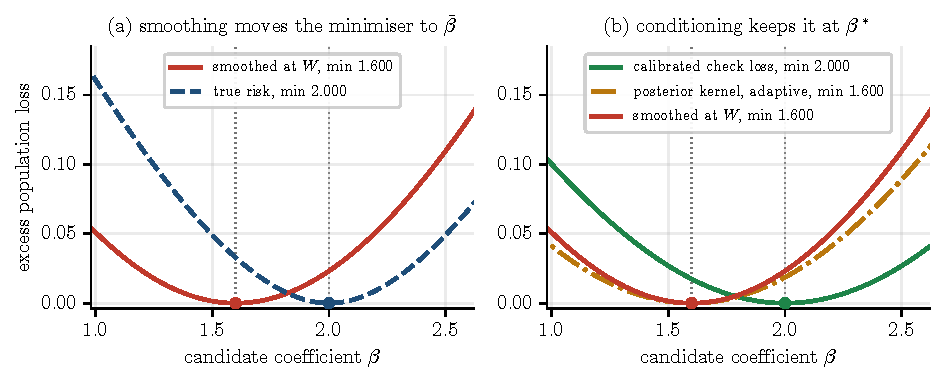
\includegraphics[width=0.82\textwidth]{../figures/fig1_loss_curves.pdf}
    \caption{Population objectives in the scalar case ($\sigma_u=0.5$, $\tau=1/2$,
    $\betas=2$, $\bbar=1.6$), computed by quadrature rather than simulated, in excess of
    each curve's own minimum. The grey dotted vertical lines mark $\bbar=1.6$ and
    $\betas=2$; each curve is marked with a dot at its minimiser, whose value is given in
    the legend. Panel (a): the smoothed loss at the raw regressor $W$ with the pilot scale
    $\sigmah$, minimised at $\bbar$, against the true risk, minimised at $\betas$.
    Panel (b): the check loss at the calibrated regressor $\muv$, minimised at $\betas$;
    the same loss with the posterior kernel $\Sxw$ at its self-consistent scale
    $\sigma_{\Sxw}(\beta)$, minimised at $\bbar$; and, for reference, the smoothed loss of
    panel (a) again, which has the same minimiser as the posterior-kernel curve. All four
    minima agree with the values predicted by Proposition~\ref{prop:exact-target} and
    Theorem~\ref{thm:calib} to $10^{-6}$.}
    \label{fig:loss}
\end{figure}

% ============================================================
\section{Discussion}
\label{sec:discussion}
% ============================================================

\paragraph{Consequences for practice.}
(i) A procedure that reports estimates from \eqref{eq:loss} with a fixed or pilot-based
scale targets $\bbar$ and should say so. (ii) Resampling-based intervals for such
estimators, the smoothed one included, cover $\bbar$, not $\betas$. (iii) For $\betas$,
calibrate the regressor and use the ordinary check loss with an intercept; the cost is that
intercept and an estimable $\Sigma_x$ (hence $\Ccal$). (iv) In small samples the smoothed
estimator's low variance can make its \emph{total} $\ell_2$ error competitive with, or
below, that of an unbiased calibrated estimator (Table~S4 of Online Resource~1), but the
advantage is finite-sample only: the bias does not shrink, and it vanishes as $n$ grows
(Table~S3 of Online Resource~1).

\paragraph{Limitations.}
The calibration identity of Theorem~\ref{thm:calib} is Gaussian: it needs linearity of
$\E[X\mid W]$ and independence of conditional mean and residual, both of which fail for
non-Gaussian $X$ or $U$.
The oracle inequality of Theorem~\ref{thm:estimated} needs row-wise accuracy of
$\hat\Ccal$, which we do not establish for growing row sparsity
(Remark~\ref{rem:spectral-not-enough}); the debiased estimator's asymptotic normality,
Theorem~\ref{thm:debias-clt}, needs the design-error penalty term to be
$o_P(n^{-1/2})$, which a known calibration achieves but the sample-covariance plug-in does
not (Proposition~\ref{prop:plugin}); and the $p>n$ implementation needs the selected
support close to the truth. Misspecification of $\Sigma_u$ affects $\Ccal$ but, by
Corollary~\ref{cor:no-conv}, cannot be repaired by convolution. \S\ref{sec:nhanes}
estimates $\Sigma_u$ from genuine replicates but cannot check it, the truth being
unknown.

\paragraph{Future work.}
First, estimating $\Ccal$ when $p\gg n$ well enough for
\eqref{eq:debias-condition}: by Proposition~\ref{prop:plugin}, finding information about
$\Sigma_x$ beyond the $n$ observations, and showing the calibrated restricted eigenvalue
condition survives the perturbation. Second, semiparametric calibration when $X\mid W$ is
not Gaussian, with the corresponding $\delta_\tau$. Third, a bias-corrected debiasing
removing the first-order effect of estimating $\Ccal$, making the plug-in usable without
independent data; conformal methods \citep{romano2019conformalized} complement it.

% ============================================================
\appendix
\section{Proofs}
\label{app:proofs}

\begin{proof}[Proof of Lemma~\ref{lem:identity}]
Let $G(r) = \E_Z[\rho_\tau(r-\sigma Z)]$ with $Z\sim\cN(0,1)$. Since
$\partial_r\rho_\tau(r-\sigma z) = \tau-\ind{r-\sigma z<0}$ and
$|\tau-\ind{\cdot}|\le1$,
$G'(r) = \E[\tau-\ind{r<\sigma Z}] = \tau-\Pbb(\sigma Z>r) = \tau-(1-\Phi(r/\sigma))
= \Phi(r/\sigma)-(1-\tau)$.
Differentiating $r[\Phi(r/\sigma)-(1-\tau)]+\sigma\phi(r/\sigma)$ gives the same
expression, so the two sides differ by a constant; as $r\to-\infty$ both behave like
$-r(1-\tau)+o(1)$, so the constant is $0$. The second derivative is
$\phi(r/\sigma)/\sigma>0$, giving strict convexity, and $\rht(r,\sigma)\to\rho_\tau(r)$ as
$\sigma\downarrow0$ follows from $G\to\rho_\tau$ by dominated convergence.
\end{proof}

\begin{proof}[Proof of Lemma~\ref{lem:bias}]
See the main text; the only ingredients are Theorem~\ref{thm:score}, the convexity and
differentiability of $L_\sigma$, and the bound
$\norm{H(\beta)}_2\le\phi(0)\lambda_{\max}(\E[WW^\top])/\sigma$ on the Hessian.
\end{proof}

\begin{proof}[Proof of Lemma~\ref{lem:perturb}]
Since $\Ccal=\Sigma_xA^{-1}=(A-\Sigma_u)A^{-1}=I-\Sigma_uA^{-1}$ and likewise
$\hat\Ccal=I-\Sigma_u\hat A^{-1}$,
\[
\hat\Ccal-\Ccal=-\Sigma_u(\hat A^{-1}-A^{-1})=-\Sigma_u\hat A^{-1}(A-\hat A)A^{-1},
\]
using $\hat A^{-1}-A^{-1}=\hat A^{-1}(A-\hat A)A^{-1}$. Taking spectral norms and using
$\|A^{-1}\|_2\le\kappa_x^{-1}$, $\|\hat A^{-1}\|_2\le2\kappa_x^{-1}$ and
$\|A-\hat A\|_2=\|\Sigma_x-\hat\Sigma_x\|_2\le\varepsilon$ gives \eqref{eq:perturb}. The
row bound follows from
$\|\mathrm{row}_j(M)\|_1\le\sqrt p\|\mathrm{row}_j(M)\|_2\le\sqrt p\|M\|_F\le p\|M\|_2$.
\end{proof}

\begin{proof}[Derivation of \eqref{eq:gamma}]
Let $V_i=X_i-{\muv}_i$, so that $W_i={\muv}_i+V_i$ and $e_i=V_i^\top\betas+\varepsilon_i$,
and let $\psi_i=\tau-\ind{e_i<\delta_\tau}$. Since ${\muv}_i$ is independent of
$(V_i,\varepsilon_i)$ and $\E[\psi_i]=0$,
$\E[W_i\psi_i]=\E[V_i\psi_i]=-\E[V_i\ind{e_i<\delta_\tau}]$. Condition on $V_i$: because
$\varepsilon_i$ is independent of $V_i$,
$\E[\ind{e_i<\delta_\tau}\mid V_i]=F_\varepsilon(\delta_\tau-V_i^\top\betas)$, so
$\E[V_i\ind{e_i<\delta_\tau}]=\E[V_ig(V_i^\top\betas)]$ with
$g(z)=F_\varepsilon(\delta_\tau-z)$. Applying Stein's lemma to the jointly Gaussian pair
$(V_i,V_i^\top\betas)$ gives
\[
\E[V_ig(V_i^\top\betas)]=\Sxw\betas\,\E[g'(V_i^\top\betas)]
=-\Sxw\betas\,\E[f_\varepsilon(\delta_\tau-V_i^\top\betas)]
=-\Sxw\betas\,f_e(\delta_\tau),
\]
because $f_e=f_\varepsilon*\cN(0,{\betas}^\top\Sxw\betas)$ is the density of $e_i$. Hence
$\E[W_i\psi_i]=f_e(\delta_\tau)\Sxw\betas$.
\end{proof}

\begin{proof}[Proof of Lemma~\ref{lem:score-control}]
Let $\psi_i^\circ = \tau-\ind{e_i<\delta_\tau}$ be the score evaluated at the truth with the
oracle design, where $e_i=Y_i-{\muv}_i^\top\betas$. We bound the two differences separately.

\emph{(i) Oracle design, oracle threshold.} By Theorem~\ref{thm:calib},
$\E[{\muv}_{ij}\psi_i^\circ]=0$ for every $j$, and $|{\muv}_{ij}\psi_i^\circ|\le|{\muv}_{ij}|$ with
${\muv}_{ij}$ sub-Gaussian of constant $K$, so Hoeffding's inequality gives
$\Pbb(|n^{-1}\sum_i{\muv}_{ij}\psi_i^\circ|>K\eta)\le2\exp(-n\eta^2/2)$. A union bound over
the $p$ coordinates and over the intercept coordinate (whose mean is
$\E[\psi_i^\circ]=\tau-F_e(\delta_\tau)=0$ and whose variance is bounded) gives
\begin{equation*}
\Big\|\frac1n\sum_{i=1}^n\binom{{\muv}_i}{1}\psi_i^\circ\Big\|_\infty \le C K\eta
\qquad\text{with probability}\quad 1-2p\,e^{-n\eta^2/2K^2}.
\end{equation*}

\emph{(ii) Estimated design, oracle threshold.} Write
$\zeta_i=({\muv}_i-{\hat{\muv}}_i)^\top\betas$, so that
$\psi_i-\psi_i^\circ=\ind{e_i<\delta_\tau}-\ind{e_i<\delta_\tau+\zeta_i}$. Taking the
conditional expectation over $e_i$ given $W_i$ and using that $f_e$ is Lipschitz with
constant $L$ near $\delta_\tau$,
\begin{equation*}
\begin{split}
\Big|\E\big[{\muv}_{ij}(\psi_i-\psi_i^\circ)\big]\Big|
&= \Big|\E\big[{\muv}_{ij}\big(F_e(\delta_\tau)-F_e(\delta_\tau+\zeta_i)\big)\big]\Big| \\
&\le \bar f\,\big|\E[{\muv}_{ij}\zeta_i]\big|
 + \frac{L\bar f}{2}\,\E\big[|{\muv}_{ij}|\zeta_i^2\big].
\end{split}
\end{equation*}
The first term is at most $\bar f K Z_nr\|\betas\|_1$, because
$|\E[{\muv}_{ij}\zeta_i]|\le\E[|{\muv}_{ij}|\,\|W_i\|_\infty]\,r\|\betas\|_1$ and
$\E|{\muv}_{ij}|\le K$; the second is at most $L\bar fK(Z_nr\|\betas\|_1)^2$, since
$|\zeta_i|\le rZ_n\|\betas\|_1$. The
deviation from this mean is controlled by Hoeffding's inequality for sub-Gaussian variables,
because $|{\muv}_{ij}(\psi_i-\psi_i^\circ)|\le|{\muv}_{ij}|$ and ${\muv}_{ij}$ is sub-Gaussian
with constant $K$. Note that the mean is of order $r$, not $\sqrt r$: the two indicator
differences cancel to first order, and it is the Lipschitz expansion above, rather than a
Cauchy--Schwarz bound on $\ind{|e_i-\delta_\tau|\le|\zeta_i|}$, that captures the
cancellation. Combining,
\begin{equation*}
\Big\|\frac1n\sum_{i=1}^n\binom{{\hat{\muv}}_i}{1}\psi_i^\circ\Big\|_\infty
\;\le\; CK\eta(1+r) + \bar f K Z_nr\|\betas\|_1 + L\bar fK\big(Z_nr\|\betas\|_1\big)^2 .
\end{equation*}

\emph{(iii) The estimated design itself.} Finally
$n^{-1}\sum_i({\hat{\muv}}_i-{\muv}_i)\psi_i = (\hat\Ccal-\Ccal)\,n^{-1}\sum_iW_i\psi_i$.
Write $S_W$ for the sup-norm of the average on the right. The $j$-th coordinate of the
difference is at most $r\,S_W$, and
$S_W\le\|\E[W_i\psi_i]\|_\infty+CK\eta$, while
$\|\E[W_i\psi_i]\|_\infty=\bmod{\gamma}_\infty(1+O(rZ_n\|\betas\|_1))$ and
$\gamma=f_e(\delta_\tau)\Sxw\betas$ is of order $\bar f\rho$ by \eqref{eq:gamma}. Adding the
three bounds gives \eqref{eq:score-control}.
\end{proof}

\begin{proof}[Proof of Proposition~\ref{prop:intercept}]
If $\E[X]=0$ then $\E[\muv]=\Ccal\E[W]=0$. The population objective
$\beta\mapsto\E[\rho_\tau(Y-\muv^\top\beta)]$ is convex with derivative at $\betas$ equal
to $-\E[\muv(\tau-\ind{e<\delta_\tau})] = -\E[\muv]\E[\tau-\ind{e<\delta_\tau}]=0$, and it
is strictly convex in a neighbourhood of $\betas$ because $f_e(\delta_\tau)>0$ and
$\E[\muv\muv^\top]\succ0$; hence $\betas$ is the unique minimiser.
\end{proof}

\begin{proof}[Proof of Theorem~\ref{thm:lowdim}]
By Theorem~\ref{thm:calib}, $(Y_i,{\muv}_i)$ follows the linear quantile regression model
\eqref{eq:correct-model} with parameter $(\betas,\delta_\tau)$. The objective
$M_n(\beta,\delta) = n^{-1}\sum_i\rho_\tau(Y_i-{\muv}_i^\top\beta-\delta)$ is convex; its
population version $M$ is twice differentiable near $(\betas,\delta_\tau)$ with gradient
zero by \eqref{eq:calib-score} and Hessian
$f_e(\delta_\tau)\E[({\muv}_i^\top,1)^\top({\muv}_i^\top,1)]$, positive definite because
$\Sigma_x\succ0$. The score contributions
$\binom{{\muv}_i}{1}(\tau-\ind{Y_i-{\muv}_i^\top\betas-\delta_\tau<0})$ are i.i.d.\ with mean
zero and covariance $\tau(1-\tau)\E[({\muv}_i^\top,1)^\top({\muv}_i^\top,1)]$, so the
Lindeberg--Feller CLT applies; the argmax continuous mapping theorem for convex objectives
\citep{pollard1991} yields $\sqrt{n}$-consistency and the stated normal limit, with the
sandwich covariance simplifying to
$\tau(1-\tau)f_e(\delta_\tau)^{-2}\E[({\muv}_i^\top,1)^\top({\muv}_i^\top,1)]^{-1}$.
\end{proof}

\begin{proof}[Proof of Theorem~\ref{thm:highdim}]
This is the case $r=0$ of Theorem~\ref{thm:estimated}: the calibration is known, so
$\hat{\muv}=\muv$ and the second and third terms in \eqref{eq:score-control} vanish. We spell
the argument out for readability. Let $\Delta=(\hat\beta-\betas,\hat\delta-\delta_\tau)$ and
$\psi_i^\circ=\tau-\ind{e_i<\delta_\tau}$.

\emph{Score.} By \eqref{eq:calib-score}, $\E[{\muv}_{ij}\psi_i^\circ]=0$ for all $j$ and
$\E[\psi_i^\circ]=0$, and the summands are sub-Gaussian with constant $K$ because
$|\psi_i^\circ|\le\max(\tau,1-\tau)\le1$. Hoeffding's inequality for sub-Gaussian
variables and a union bound over the $p+1$ coordinates of
$\binom{{\muv}_i}{1}$ give
$\|n^{-1}\sum_i\binom{{\muv}_i}{1}\psi_i^\circ\|_\infty\le CK\sqrt{\log(p/\epsilon)/n}$ with
probability at least $1-\epsilon$. With $\lambda=C_0\sqrt{\log(p/\epsilon)/n}$ and $C_0$
large, the penalty therefore dominates twice the score.

\emph{Cone.} Comparing the objective at $(\hat\beta,\hat\delta)$ and at
$(\betas,\delta_\tau)$, using the convexity of $\rho_\tau$ and the subgradient bound just
obtained, yields $\|\Delta_{S^c}\|_1\le3\|\Delta_S\|_1$ by the standard argument
\citep[Lemma 3]{belloni2011l1}; the intercept is unpenalised, which is why the cone
constraint is imposed on $\beta$ only.

\emph{Rates.} By Assumption~\ref{ass:re-est} with $\hat{\muv}=\muv$ and the basic inequality,
$\frac{\kappa}{2}\|\Delta\|_2^2\le\frac{3\lambda}{2}\sqrt s\|\Delta\|_2+\lambda^2s$, so
$\|\Delta\|_2\le6\lambda\sqrt s/\kappa$, and
$\|\Delta\|_1\le4\sqrt s\|\Delta\|_2\le24\lambda s/\kappa$. Substituting
$\lambda\asymp\sqrt{\log p/n}$ gives the three displays. Finally, the contrast with the
smoothed loss is that there the corresponding score at the truth has mean
$\Sigma_u\betas\,d(\sigma)\neq0$ by Theorem~\ref{thm:score}, so no choice of $\lambda$ can
make the linear term small: the argument fails at its first step, not at its constants.
\end{proof}

\begin{proof}[Proof of Theorem~\ref{thm:debias-clt}]
Write ${\tilde{\muv}}_i=({\muv}_i^\top,1)^\top$ and
${\tilde{\hat{\muv}}}_i=({\hat{\muv}}_i^\top,1)^\top$. Let
$\hat S=n^{-1}\sum_i{\tilde{\hat{\muv}}}_i\psi_i$ with
$\psi_i=\tau-\ind{Y_i-{\hat{\muv}}_i^\top\hat\beta-\hat\delta<0}$, and write
$\psi_i^\circ=\tau-\ind{e_i<\delta_\tau}$,
$S^\circ=n^{-1}\sum_i{\tilde{\muv}}_i\psi_i^\circ$,
$\Delta=\hat\beta-\betas$, and $\Delta_\delta=\hat\delta-\delta_\tau$.

\emph{Step 1 (decomposition).} By \eqref{eq:debias},
$\hat b_j-\beta^*_j=\hat\Theta_{j\cdot}\hat S+\Delta_j$, and
$\hat S=S^\circ+R$ with
$R=n^{-1}\sum_i({\tilde{\hat{\muv}}}_i-{\tilde{\muv}}_i)\psi_i^\circ
+n^{-1}\sum_i{\tilde{\muv}}_i(\psi_i-\psi_i^\circ)
+n^{-1}\sum_i({\tilde{\hat{\muv}}}_i-{\tilde{\muv}}_i)(\psi_i-\psi_i^\circ)
=R_1+R_2+R_3$.

\emph{Step 2 (the estimated-design part of the score).} For $R_1$, the first block of$n^{-1}\sum_i({\tilde{\hat{\muv}}}_i-{\tilde{\muv}}_i)\psi_i^\circ$ is
$(\hat\Ccal-\Ccal)n^{-1}\sum_iW_i\psi_i^\circ$, and the second block is zero. Its mean is
$(\hat\Ccal-\Ccal)\gamma$, up to a factor $1+O_P(rZ_n\|\betas\|_1)$. Since
$\gamma=f_e(\delta_\tau)\Sxw\betas$ by \eqref{eq:gamma} obeys
$\|\gamma\|_1\le\bar f\|\Sxw\|_2\|\betas\|_1$, that mean is of order
$r_n\|\betas\|_1$. The deviation around it is $O_P(r_n\sqrt{\log p/n})$ by Hoeffding's
inequality, because $\|(\hat\Ccal-\Ccal)W_i\|_\infty\le r_nZ_n$. Hence
\[
\|R_1\|_\infty=O_P\big(r_n\|\betas\|_1+r_n\sqrt{\log p/n}\big),
\]
and the first two terms of \eqref{eq:debias-condition} control it.

For $R_2$, put $v_i={\tilde{\hat{\muv}}}_i^\top\Delta$ and
$\zeta_i=({\hat{\muv}}_i-{\muv}_i)^\top\betas$, so that
$\psi_i-\psi_i^\circ=\ind{e_i<\delta_\tau}-\ind{e_i<\delta_\tau+v_i+\Delta_\delta}$.
Conditionally on the design,
$\E[\psi_i-\psi_i^\circ\mid\mathcal{D}]
= F_e(\delta_\tau+v_i+\Delta_\delta)-F_e(\delta_\tau)
= f_e(\delta_\tau)(v_i+\Delta_\delta)+O\big(L(v_i+\Delta_\delta)^2\big)$,
the second equality being the Lipschitz property of $f_e$; note
$|v_i|\le\|{\tilde{\hat{\muv}}}_i\|_1\|\Delta\|_1$ and
$|\zeta_i+\Delta_\delta|\le Z_nr_n\|\betas\|_1+\|\Delta_\delta\|$. Summing,
\[
\begin{split}
\E[R_2\mid\mathcal{D}]
=f_e(\delta_\tau)\Big\{n^{-1}\sum_i{\tilde{\muv}}_i{\tilde{\hat{\muv}}}_i^\top\Delta
+\Delta_\delta\,n^{-1}\sum_i{\tilde{\muv}}_i\Big\}\\
+O_P\big(L(1+Z_n)Z_n\|\Delta\|_1^2+LZ_n\|\Delta\|_1\|\Delta_\delta\|\big).
\end{split}
\]
The first bracket is the population Hessian, evaluated at the estimated design, times
$\Delta$: writing $\hat H_0=f_e(\delta_\tau)n^{-1}\sum_i{\tilde{\hat{\muv}}}_i{\tilde{\hat{\muv}}}_i^\top$,
the display equals $\hat H_0\Delta+O_P(\|\Delta\|_1)$ and, since
$n^{-1}\sum_i{\tilde{\muv}}_i$ has $\ell_\infty$ norm $O_P(\sqrt{\log p/n})$, the
$\Delta_\delta$ term is $O_P(\|\Delta_\delta\|\sqrt{\log p/n})$. For the deviation of $R_2$
around its conditional mean, independence across $i$ and $|\psi_i-\psi_i^\circ|\le1$ give
\[
\Big(\sum_i\|{\tilde{\muv}}_i\|_1^2\,\E\big[(\psi_i-\psi_i^\circ)^2\big]\Big)^{1/2}
\le K\Big(\sum_i\E|\psi_i-\psi_i^\circ|\Big)^{1/2},
\]
and, by the Lipschitz expansion of $F_e$ used above,
$n^{-1}\sum_i\E|\psi_i-\psi_i^\circ|=O(\|\Delta\|_1+|\Delta_\delta|)$, because
$n^{-1}\sum_i|v_i|\le\big(n^{-1}\sum_iv_i^2\big)^{1/2}$, so the deviation is
$O_P\big(n^{-1/2}(\|\Delta\|_1+|\Delta_\delta|)^{1/2}\big)=o_P(n^{-1/2})$: the expectation of
the indicator difference vanishes with the perturbation, and it is that, rather than the bound
$|\psi_i-\psi_i^\circ|\le1$, which makes the fluctuation negligible.
Finally $\|R_3\|_\infty\le r_nZ_n\cdot n^{-1}\sum_i|\psi_i-\psi_i^\circ|
=O_P(r_nZ_n(\|\Delta\|_1+\sqrt{\log p/n}))$ by the same Lipschitz bound.

Adding the three pieces,
\begin{equation}
\hat S=S^\circ+\hat H_0\Delta+R,
\qquad
\|R\|_\infty=o_P(n^{-1/2})+O_P\big((1+Z_n)Z_n\|\Delta\|_1^2\big),
\label{eq:debias-expansion}
\end{equation}
where the $o_P(n^{-1/2})$ collects the design terms, whose size is
$O_P(\rho r_n+r_n\|\betas\|_1+r_n\sqrt{\log p/n})$ plus the $R_2$ fluctuation, all
$o_P(n^{-1/2})$ by \eqref{eq:debias-condition}; and the $O_P$ term is the second-order
remainder of the indicator expansion, also $o_P(n^{-1/2})$ by the third clause of
\eqref{eq:debias-condition}, which is stated with the factor $1+Z_n$ that the weighted sum
produces; the bound $n^{-1}\sum_i v_i^2\le C_3s\lambda^2/\kappa$ of
Theorem~\ref{thm:estimated} is what lets the weighted sum be bounded by $(1+Z_n)$ times its
largest term.

\emph{Step 3 (the Newton remainder).} Inserting \eqref{eq:debias-expansion} into Step 1,
\[
\hat b_j-\beta^*_j
=\hat\Theta_{j\cdot}S^\circ+\big(e_j'-\hat\Theta_{j\cdot}\hat H_0\big)\Delta
+\hat\Theta_{j\cdot}R .
\]
By \eqref{eq:nodewise} and $\|\hat\Theta_{j\cdot}\|_1=O_P(1)$,
$\|e_j'-\hat\Theta_{j\cdot}\hat H_0\|_\infty\le\|e_j'-\hat\Theta_{j\cdot}\hat H\|_\infty
+\|\hat\Theta_{j\cdot}\|_1\|\hat H-\hat H_0\|_\infty
=O_P(\sqrt{\log p/n})+O_P(h+(nh)^{-1/2})$, and
$\|\hat H-\hat H_0\|_\infty=O_P(h+(nh)^{-1/2})$ is the bias and variance of the kernel
smoother at bandwidth $h$; with $h\to0$ and $nh\to\infty$ the second term is
$o_P(\sqrt{\log p/n})$, so
$|(e_j'-\hat\Theta_{j\cdot}\hat H_0)\Delta|=O_P(\sqrt{\log p/n}\,\|\Delta\|_1)
=o_P(n^{-1/2})$ by $\|\Delta\|_1=o_P((\log p)^{-1/2})$. The last piece is
$\hat\Theta_{j\cdot}R=O_P(\|R\|_\infty)=o_P(n^{-1/2})$ by \eqref{eq:debias-expansion}.
Hence
$\sqrt n(\hat b_j-\beta^*_j)=\sqrt n\,\hat\Theta_{j\cdot}S^\circ+o_P(1)$.

\emph{Step 4 (the linear term).} Write
$\hat\Theta_{j\cdot}S^\circ=\Theta_{j\cdot}S^\circ+(\hat\Theta_{j\cdot}-\Theta_{j\cdot})S^\circ$.
By \eqref{eq:nodewise} and $\hat\Theta_{j\cdot}-\Theta_{j\cdot}
=-\big(\hat\Theta_{j\cdot}(\hat H-H_0)+(\hat\Theta_{j\cdot}\hat H_0-e_j')\big)\Theta$,
$\|\hat\Theta_{j\cdot}-\Theta_{j\cdot}\|_1=O_P(\sqrt{\log p/n}+h+(nh)^{-1/2})
=O_P(\sqrt{\log p/n})$, so the second term is
$O_P(\sqrt{\log p/n}\|S^\circ\|_\infty)=O_P(\log p/n)=o_P(n^{-1/2})$, where
$\|S^\circ\|_\infty=O_P(\sqrt{\log p/n})$ is Hoeffding's inequality for the sub-Gaussian
summands ${\tilde{\muv}}_{ij}\psi_i^\circ$. It remains to treat
$\sqrt n\,\Theta_{j\cdot}S^\circ=n^{-1/2}\sum_i\Theta_{j\cdot}{\tilde{\muv}}_i\psi_i^\circ$.
The summands are independent across $i$, and
$\E[\psi_i^\circ\mid{\muv}_i]=0$ because $e_i$ is independent of ${\muv}_i$ and
$F_e(\delta_\tau)=\tau$ \eqref{eq:calib-score}; their conditional variance is
$\tau(1-\tau)$, so
$\sum_i\E[(\Theta_{j\cdot}{\tilde{\muv}}_i\psi_i^\circ)^2]
=\tau(1-\tau)\Theta_{j\cdot}\E[\tilde{\muv}{\tilde{\muv}}^\top]\Theta_{j\cdot}^\top$.
Lindeberg's condition holds: $\max_i|\Theta_{j\cdot}{\tilde{\muv}}_i|\le\|\Theta_{j\cdot}\|_1
\max_i\|{\tilde{\muv}}_i\|_\infty=O_P(\sqrt{\log(np)})$, so
$\max_i|n^{-1/2}\Theta_{j\cdot}{\tilde{\muv}}_i\psi_i^\circ|=o_P(1)$, and truncating at
$\epsilon\sqrt n$ leaves a remainder bounded by
$O(\E[\|\tilde{\muv}\|^2\ind{\|\tilde{\muv}\|>\epsilon\sqrt n/\|\Theta_{j\cdot}\|_1}])=o(1)$
by the sub-Gaussian tail. Hence
\[
\sqrt n\,\Theta_{j\cdot}S^\circ\ \rightsquigarrow\
\cN\Big(0,\ \tau(1-\tau)\,\Theta_{j\cdot}\E[\tilde{\muv}{\tilde{\muv}}^\top]\Theta_{j\cdot}^\top\Big).
\]
Since $\Theta=(f_e(\delta_\tau)\E[{\tilde{\muv}}{\tilde{\muv}}^\top])^{-1}$ by
Theorem~\ref{thm:lowdim}, the variance equals
\[
\tau(1-\tau)\,f_e(\delta_\tau)^{-2}\,
\Big(\E\big[{\tilde{\muv}}{\tilde{\muv}}^\top\big]^{-1}\Big)_{jj},
\]
which is \eqref{eq:debias-clt}. Together with the consistency of the sandwich estimator this
gives Slutsky's statement of the theorem.
\end{proof}

\begin{proof}[Proof of Proposition~\ref{prop:plugin}]
Since $\hat A=\hat\Sigma_x+\Sigma_u$ and $A=\Sigma_x+\Sigma_u$, we have
$\hat A-A=D$, and Lemma~\ref{lem:perturb} gives
$\hat\Ccal-\Ccal=-\Sigma_u(\hat A^{-1}-A^{-1})=\Sigma_u\hat A^{-1}DA^{-1}$.
Under $\|\hat\Sigma_x-\Sigma_x\|_2\le\kappa_x/2$ we have $\hat A\succeq\frac12A$, so the
rows of $\hat A^{-1}$ have $\ell_1$ norm at most $2b$, and
\[
\begin{split}
\big\|(\hat\Ccal-\Ccal)_{j\cdot}\big\|_1
&=\big\|e_j^\top\Sigma_u\hat A^{-1}DA^{-1}\big\|_1\\
&\le\big\|e_j^\top\Sigma_u\hat A^{-1}\big\|_1\,
\max_k\big\|(DA^{-1})_{k\cdot}\big\|_1
\le 2\sigma_{\max}(\Sigma_u)\,b^2s_0\varepsilon_n,
\end{split}
\]
because $\|(DA^{-1})_{k\cdot}\|_1\le\sum_l|D_{kl}|\|(A^{-1})_{l\cdot}\|_1
\le b\|D_{k\cdot}\|_1\le bs_0\varepsilon_n$. That is \eqref{eq:plugin}. For the sample
covariance, $\max_{k,l}|D_{kl}|=O_P(\sqrt{\log p/n})$ by the sub-Gaussian tail of
$W_{ik}W_{il}-\E[W_{ik}W_{il}]$, and $Z_n=\max_i\|W_i\|_\infty\asymp\sqrt{\log p}$; hence
$Z_nr_n\|\betas\|_1\gtrsim s_0(\log p)\|\betas\|_1/\sqrt n$, and multiplying by $\sqrt n$
gives $s_0(\log p)\|\betas\|_1$, which does not vanish as soon as $\log p$ grows with $n$.
This is the scale of the violation of \eqref{eq:debias-condition}, not a claim that the bias
of $\hat b_j$ equals it: the design terms are what the condition rules out, and
Table~\ref{tab:plugin} measures how much of them shows up as bias in the experiment there.
\end{proof}

\begin{proof}[Proof of Theorem~\ref{thm:score}]
[Proof]
Condition on $\varepsilon_i=e$. The map
$z\mapsto h(z) = \Phi((e-z)/\sigma)-(1-\tau)$ is Lipschitz, so Stein's lemma for
$(U_{ij},U_i^\top\betas)$ gives
$\E[U_{ij}h(U_i^\top\betas)] = (\Sigma_u\betas)_j\,\E[h'(U_i^\top\betas)]
= -(\Sigma_u\betas)_j\,\E[\phi((e-U_i^\top\betas)/\sigma)]/\sigma$.
Since $U_i^\top\betas\sim\cN(0,\sigma^{*2})$, this is $-(\Sigma_u\betas)_j g(e)$, the
density of $e+\cN(0,\sigma^{*2}+\sigma^2)$ at $0$, so integrating over $e$ gives
$\E[U_{ij}\psit(r_i^*,\sigma)] = -(\Sigma_u\betas)_j d(\sigma)$ with
$d(\sigma) = \E[g(\varepsilon_i)]$. As $\psit(r_i^*,\sigma)$ depends only on
$(\varepsilon_i,U_i)$ and $\E[X_i]=0$, $\E[X_{ij}\psit(r_i^*,\sigma)] = 0$, and
$W_i = X_i+U_i$ gives \eqref{eq:score-bias}. Positivity follows from
$f_\varepsilon(0)>0$ and continuity.
\end{proof}

\begin{proof}[Proof of Theorem~\ref{thm:kernel-class}]
With $\psi_G(r) = F_G(r)-(1-\tau)$ and $h(z) := F_G(\varepsilon_i-z)-(1-\tau)$, so
$h'(z) = -g(\varepsilon_i-z)$, conditioning on $\varepsilon_i$ and applying Stein's lemma
to $(U_{ij},U_i^\top\betas)$ gives
$\E[U_{ij}\psi_G(r_i^*)] = -(\Sigma_u\betas)_j\E[g(\varepsilon_i-U_i^\top\betas)]
= -(\Sigma_u\betas)_j D_G$, and $\E[X_{ij}\psi_G(r_i^*)]=0$ as before. Positivity of
$D_G$ follows from $g(0)>0$ and continuity; for $G=\cN(0,\sigma^2)$, $g(x)=\phi(x/\sigma)/\sigma$
gives $D_G = \E[\phi((\varepsilon_i-Z_i)/\sigma)]/\sigma = d(\sigma)$ by the proof of
Theorem~\ref{thm:score}.
\end{proof}

\begin{proof}[Proof of Theorem~\ref{thm:adaptive}]
Differentiation under the expectation is valid ($\psit,\phi$ bounded,
$\E\|W_i\|<\infty$). At $\beta=\betas$ the first term is
$\Sigma_u\betas\,d_M$ by Theorem~\ref{thm:score} with $\sigma=s_M$. For the second,
conditioning on $\varepsilon_i$ and using $U_i^\top\betas\sim\cN(0,\sigma^{*2})$,
\[
\E\big[\phi((\varepsilon_i-U_i^\top\betas)/s_M)\big]
= \int\phi\Big(\frac{\varepsilon_i-z}{s_M}\Big)\frac{1}{\sigma^*}\phi\Big(\frac{z}{\sigma^*}\Big)dz
= s_M\,\phi_{\sqrt{\sigma^{*2}+s_M^{2}}}(\varepsilon_i),
\]
the convolution of $\cN(0,s_M^{2})$ and $\cN(0,\sigma^{*2})$; integrating over
$\varepsilon_i$ and using symmetry gives $\E[\phi(r_i^*/s_M)] = s_M\,d_M$. Multiplying by
$M\betas/s_M$ and adding the first term gives \eqref{eq:adaptive}.
\end{proof}

\begin{proof}[Proof of Proposition~\ref{prop:target}]
By the mean value theorem in its integral form,
$\nabla L(\betas+v) = g+Hv+R(v)$ with
$\|R(v)\|\le\frac\Lambda2\|v\|^2$ for $\|v\|\le\eta$. Since $0=\nabla L(\bbar_\sigma)$,
\[
\bbar_\sigma-\betas = -H^{-1}g - H^{-1}R(\bbar_\sigma-\betas),
\]
so with $u = \|\bbar_\sigma-\betas\|$ and
$m=\|H^{-1}g\|\le\|g\|/\kappa$, $u \le m+\frac{\Lambda}{2\kappa}u^2$. Hypothesis (iii)
gives $\frac{2\Lambda}{\kappa}m\le\frac14$, so $u\le2m$ and substituting back gives the
first bound. Strict convexity on $B(\betas,\eta)$ gives uniqueness.
\end{proof}

\begin{proof}[Proof of Corollary~\ref{cor:no-conv}]
The computation of Theorem~\ref{thm:score} uses only $W = X+U$ with
$U\sim\cN(0,\Sigma_u)$, so replacing $\Sigma_u$ by $\Sigma_k$ is the same calculation, and
$\E[X\psit]=0$ is unchanged. Displacement follows from Lemma~\ref{lem:bias} with
$\Sigma_k$.
\end{proof}

\begin{proof}[Proof of Proposition~\ref{prop:posterior-adaptive}]
Write $\xi_i=X_i-\Ccal W_i$, so $\E[\xi_i\mid W_i]=0$ and
$\mathrm{Var}(\xi_i\mid W_i)=\Sxw$, and let $Z\sim\cN(0,1)$ be
independent of $(X_i,U_i,\varepsilon_i)$. Since $\rht(r,\sigma)=\E[\rho_\tau(r-\sigma Z)]$,
\begin{equation}
Y_i-{\muv}_i^\top\beta
=(\Ccal W_i)^\top(\betas-\beta)+{\betas}^\top\xi_i+\varepsilon_i,
\qquad
L_{\mathrm{cal}}(\beta)=\E\big[\rho_\tau\big(\varepsilon_i+G_i(\beta)\big)\big],
\label{eq:cal-gauss}
\end{equation}
where $G_i(\beta)\sim\cN(0,\varsigma^2(\beta))$ is independent of $\varepsilon_i$ and
\begin{equation}
\varsigma^2(\beta)=(\betas-\beta)^\top\Ccal(\Sigma_x+\Sigma_u)\Ccal^\top(\betas-\beta)
+{\betas}^\top\Sxw\betas+\beta^\top\Sxw\beta .
\label{eq:cal-scale}
\end{equation}
Indeed, conditional on $W_i$ the term ${\betas}^\top\xi_i-\sigma_{\Sxw}(\beta)Z$ is centred
Gaussian with variance ${\betas}^\top\Sxw\betas+\beta^\top\Sxw\beta$ irrespective of $W_i$,
hence independent of $(\Ccal W_i)^\top(\betas-\beta)$, itself centred Gaussian with
covariance $\Ccal(\Sigma_x+\Sigma_u)\Ccal^\top$. For $N\sim\cN(0,1)$ independent of
$\varepsilon_i$,
\[
\frac{\partial}{\partial\sigma}\E\big[\rho_\tau(\varepsilon_i+\sigma N)\big]
=\E\big[\psit(\varepsilon_i+\sigma N)N\big]
=\E\big[\phi(\varepsilon_i/\sigma)\big]>0,
\]
using $\E[N\ind{N<c}]=-\phi(c)$; so \eqref{eq:cal-gauss} is
strictly increasing in $\varsigma(\beta)$, and minimising $L_{\mathrm{cal}}$ is the same as
minimising $\varsigma^2$. Finally
$\Ccal(\Sigma_x+\Sigma_u)\Ccal^\top=\Sigma_x(\Sigma_x+\Sigma_u)^{-1}\Sigma_x
=\Sigma_x-\Sxw$, so \eqref{eq:cal-scale} has gradient $2\Sigma_x(\beta-\bbar)$, which
vanishes only at $\bbar$, and $\Sigma_x\succ0$.
\end{proof}

\begin{proof}[Proof of Corollary~\ref{cor:same-target}]
For $Z\sim\cN(0,\sigma^{*2})$ and $U_i^\top\betas$ jointly Gaussian with
$U_{ij}$, $\E[U_{ij}\ind{U_i^\top\betas>\varepsilon_i}]
= (\Sigma_u\betas)_j\,\phi_{\sigma^*}(\varepsilon_i)$
by the conditional-expectation formula for jointly Gaussian variables
($\E[U_{ij}\mid U_i^\top\betas=z] = (\Sigma_u\betas)_j z/\sigma^{*2}$ and
$\E[Z\ind{Z>\varepsilon}] = \sigma^{*2}\phi_{\sigma^*}(\varepsilon)$). Hence
$\E[U_{ij}(\tau-\ind{r_i^*<0})] = -(\Sigma_u\betas)_j\E[\phi_{\sigma^*}(\varepsilon_i)]
= -(\Sigma_u\betas)_j(\cN(0,\sigma^{*2})*f_\varepsilon)(0)$,
while $\E[X_{ij}(\tau-\ind{r_i^*<0})]=0$ as before, and
Proposition~\ref{prop:target} with $d_{\mathrm{naive}}$ in place of $d(\sigma)$ gives the
target statement.
\end{proof}

\begin{proof}[Proof of Proposition~\ref{prop:exact-target}]
Write the residual at a candidate $\beta$ as
$\varepsilon_i+X_i^\top(\betas-\beta)-U_i^\top\beta-Z\sigma$, where $Z\equiv0$ and
$\sigma=0$ for the naive risk and $Z\sim\cN(0,1)$ is independent of everything for the
smoothed ones, with $\sigma$ replaced by $\sigma_M(\beta)$ in case (iii). Its
non-$\varepsilon$ part is centred Gaussian, $(X_i,U_i,Z)$ being Gaussian with
$\E[X_i]=\E[U_i]=0$, with variance
$s^2(\beta)=(\betas-\beta)^\top\Sigma_x(\betas-\beta)+\beta^\top\Sigma_u\beta+\sigma^2$ in
cases (i)--(ii) and $\beta^\top(\Sigma_u+M)\beta$ in place of $\beta^\top\Sigma_u\beta+\sigma^2$
in case (iii), independent of $\varepsilon_i$. The risk
$\E[\rho_\tau(\varepsilon_i+s(\beta)Z_0)]$ depends on $\beta$ only through $s(\beta)$, and
$s\mapsto\E[\rho_\tau(\varepsilon_i+sZ_0)]$ is strictly increasing by the proof of
Proposition~\ref{prop:posterior-adaptive}, so the risk is a strictly increasing function of
$s^2(\beta)$ and shares its minimiser, unique because $s^2$ is a strictly convex quadratic
with gradient $2\big[(\Sigma_x+\Sigma_u+M)\beta-\Sigma_x\betas\big]$ vanishing exactly at
the values stated.
\end{proof}

\begin{proof}[Proof of Theorem~\ref{thm:calib}]
[Proof]
For jointly Gaussian vectors, ${\muv}_i=\E[X_i\mid W_i]$ and $V_i = X_i-{\muv}_i$ are
independent with $V_i\sim\cN(0,\Sxw)$. Since ${\muv}_i$ is a function of $W_i$ and
$\varepsilon_i$ is independent of $(X_i,U_i)$, $e_i$ depends on $(V_i,\varepsilon_i)$ alone
and so is independent of ${\muv}_i$; hence $Y_i = {\muv}_i^\top\betas+e_i$ and
$Q_\tau(Y_i\mid{\muv}_i) = {\muv}_i^\top\betas+Q_\tau(e_i)$, which is
\eqref{eq:correct-model} with $\delta_\tau = Q_\tau(V_i^\top\betas+\varepsilon_i)$. For
\eqref{eq:calib-score}, the first $p$ coordinates vanish because
$\E[{\muv}_i(\tau-\ind{e_i<\delta_\tau})] = \E[{\muv}_i]\,\E[\tau-\ind{e_i<\delta_\tau}]=0$
(independence and $\E[X_i]=0$), and the last coordinate is
$\tau-\Pbb(e_i<\delta_\tau)=0$ by definition of $\delta_\tau$.
\end{proof}

\begin{proof}[Proof of Theorem~\ref{thm:estimated}]
\emph{Step 1 (the penalty dominates the score).}
Apply Lemma~\ref{lem:score-control} with
$\eta\asymp\sqrt{\log(p/\epsilon_n)/n}$. Its
right-hand side is bounded by $C_0\lambda$ for $\lambda$ as in \eqref{eq:lambda-est}: the
factor $(1+r)$ on $\eta$ and on $\bar fZ_nr\|\betas\|_1$ is absorbed into $C_0$ because
$r\to0$; $r\bar f\rho$ is the $\rho r$ of \eqref{eq:lambda-est}; and
Assumption~\ref{ass:small-design} bounds $r(\rho+rZ_n\|\betas\|_1)$ by
$c_0\sqrt{\log p/n}$ and the Lipschitz remainder $O(\alpha^2)$,
$\alpha=Z_nr\|\betas\|_1\le c_1$, by $O(\alpha)$, so both are absorbed.
Every term vanishes as $r\to0$, as it must: at $r=0$ the score is mean-zero
(Theorem~\ref{thm:calib}). Hence $\|S\|_\infty\le\lambda/2$ with probability at
least $1-\epsilon_n-2p^{-c}$, as the cone argument below requires.

\emph{Step 2 (restricted eigenvalue transfers).} For $\theta\in(0,1)$ and all
$a,b\in\R$, $(a+b)^2\ge(1-\theta)a^2-\frac{1-\theta}{\theta}b^2$; apply this to
$a={\muv}_i^\top\Delta$, $b=({\hat{\muv}}_i-{\muv}_i)^\top\Delta$ with $\theta=1/4$ and
average over $i$. Since $|b|\le r\|W_i\|_\infty\|\Delta\|_1\le rZ_n\|\Delta\|_1$ and
$\|\Delta\|_1\le4\sqrt s\|\Delta\|_2$ on the cone,
$\frac1n\sum_i b_i^2\le r^2Z_n^2\|\Delta\|_1^2\le16r^2Z_n^2s\|\Delta\|_2^2$, so
\begin{equation*}
\frac1n\sum_i({\hat{\muv}}_i^\top\Delta)^2
\;\ge\;\Big(\frac34\kappa-3\cdot16r^2Z_n^2s\Big)\|\Delta\|_2^2
\;\ge\;\frac{9}{16}\kappa\|\Delta\|_2^2
\;\ge\;\frac\kappa2\|\Delta\|_2^2
\end{equation*}
by Assumption~\ref{ass:small-design}, so the transfer constant
$(\sqrt\kappa-4rZ_n\sqrt s)^2$ is at least $9\kappa/16$.

\emph{Step 3 (basic inequality and the cone).} Let
$\Delta=(\hat\beta-\betas,\hat\delta-\delta_\tau)$ and
$Q_n(\beta,\delta)=n^{-1}\sum_i\rho_\tau(Y_i-{\hat{\muv}}_i^\top\beta-\delta)$. Comparing
$Q_n(\hat\beta,\hat\delta)+\lambda\|\hat\beta\|_1$ with the value at $(\betas,\delta_\tau)$,
convexity of $\rho_\tau$ and the subgradient bound of Step 1 give the
cone property $\|\Delta_{S^c}\|_1\le3\|\Delta_S\|_1$ exactly as in
\citet[Lemma 3]{belloni2011l1}. Knight's identity, with
$v_i={\hat{\muv}}_i^\top\Delta$ and $F_e$ the distribution function of $e_i$, whose
$\tau$-quantile is $\delta_\tau$, gives
\begin{equation*}
\rho_\tau(e_i-v_i)-\rho_\tau(e_i)
= -v_i\big(\tau-\ind{e_i<\delta_\tau}\big)+\int_0^{v_i}\big(F_e(\delta_\tau+s)-F_e(\delta_\tau)\big)\,ds ,
\end{equation*}
so the loss difference dominates $\frac{\underline f}{2}v_i^2$ up to the linear term and a
third-order remainder ($\underline f$ bounds $f_e$ from below near $\delta_\tau$), and
Young's inequality absorbs the self-normalised empirical process into
$\lambda^2s$. Combining the pieces,
\begin{equation*}
\frac{\kappa}{2}\|\Delta\|_2^2 \;\le\; \frac1n\sum_{i=1}^n
\big({\hat{\muv}}_i^\top(\hat\beta-\betas)\big)^2
\;\le\; \frac{3\lambda}{2}\|\Delta_S\|_1+\lambda^2s ,
\end{equation*}
the first inequality by Step 2, the second by the basic inequality with
$\|\Delta_S\|_1\le\sqrt s\|\Delta\|_2$. Solving the resulting quadratic inequality,
\[
\|\Delta\|_2\le\frac{6\lambda\sqrt s}{\kappa},
\qquad
\|\Delta\|_1\le4\sqrt s\|\Delta\|_2\le\frac{24\lambda s}{\kappa},
\]
and substituting back gives the prediction bound, proving the three displays with
$C_1=6$, $C_2=24$ and $C_3=18/\kappa$ after absorbing constants. The final statement
follows because $\lambda\asymp C_0\sqrt{\log p/n}$ when $r\asymp\sqrt{\log p/n}$ and
$rZ_n\|\betas\|_1\lesssim\sqrt{\log p/n}$, the latter being the condition
$s\log p\log(np)\ll n$ under sub-Gaussianity of $W$.
\end{proof}

\section{Computation}
\label{app:computation}

All estimators are fitted by the same damped-Newton or proximal-gradient routine applied to
the smoothed loss with bandwidth $h$; methods differ only in the design ($W$ versus
$\muv$) and in whether $h$ is a computational constant ($h=0.01$) or the measurement-error
scale ($h=\sigmah$). For the check-loss methods the smoothing bias is
$O(h^2)=10^{-4}$, which we verified against an exact linear-programming solution on small
problems. The population targets of Table~\ref{tab:targets} are computed without any
optimiser: the unpenalised scalar quantile problem is solved by exact subgradient
root-finding (the subgradient is monotone and available in $O(\log n)$ from sorted arrays),
and the intercept version by profiling over the slope with the intercept equal to the
empirical $\tau$-quantile of the residuals, which is exact by partial minimisation.

\section{Supplementary numerical results}
\label{app:numerics}

This appendix collects the numerical studies that support the theory but are
not needed for the argument of the paper.

\subsection{Population targets of the calibration-based estimators}
\label{sec:targets-calib-si}

Table~\ref{tab:targets_calib} reports the population targets of the
calibration-based estimators, on the same designs as Table~\ref{tab:targets}.

\begin{table}[ht]
\centering
\footnotesize
\caption{Population targets of the calibration-based estimators (same designs as Table~\ref{tab:targets}). ``RC'' regresses $Y$ on $\muv=\Ccal W$; ``RC$+$int'' adds an intercept. Both recover $\betas$ within Monte-Carlo error, and the fitted intercept agrees with the predicted quantile shift $\delta_\tau$ of Theorem~\ref{thm:calib}. For reference the exact value $\betas=2$ and the oracle fit on the clean $X$ are shown.}
\label{tab:targets_calib}
\begin{tabular}{lcccccc}
\toprule
$\sigma_u$ & $\tau$ & RC & RC$+$int & fitted intercept & predicted $\delta_\tau$ & oracle \\
\midrule
0.1 & 0.3 & 1.998 & 1.998 & -0.0173 & -0.0166 & 1.998 \\
0.1 & 0.5 & 2.002 & 2.002 & +0.0059 & +0.0001 & 2.001 \\
0.1 & 0.7 & 1.999 & 1.999 & +0.0159 & +0.0170 & 1.999 \\
\midrule
0.3 & 0.3 & 1.997 & 1.997 & -0.1108 & -0.1110 & 1.997 \\
0.3 & 0.5 & 2.005 & 2.005 & +0.0030 & +0.0004 & 2.001 \\
0.3 & 0.7 & 1.999 & 2.001 & +0.1135 & +0.1118 & 1.998 \\
\midrule
0.5 & 0.3 & 2.000 & 2.003 & -0.2294 & -0.2293 & 2.000 \\
0.5 & 0.5 & 1.996 & 1.996 & -0.0034 & -0.0010 & 2.003 \\
0.5 & 0.7 & 2.002 & 2.003 & +0.2269 & +0.2286 & 2.000 \\
\bottomrule
\end{tabular}
\end{table}


\subsection{The score check}
\label{sec:scorecheck}

Theorem~\ref{thm:score} is a statement about a population mean and can be checked
directly. Table~\ref{tab:score} reports Monte-Carlo estimates of
$\E[W_{i1}\psit(r_i^*,\sigma^*)]$ and of the calibrated score
$\E[{\muv}_{i1}(\tau-\ind{e_i<\delta_\tau})]$ at the truth. The smoothed score is non-zero
with $t$-statistics in the tens and matches the analytic value $-(\Sigma_u\betas)_1d(\sigma^*)$;
the calibrated score is indistinguishable from zero. This is the empirical content of the
distinction between the two sections: one score is biased by $\Theta(\rho)$, the other is
exactly unbiased.

\begin{table}[ht]
\centering
\small
\caption{Population score at the truth, $\E[W_{i1}\psit(r_i^*,\sigma^*)]$ (smoothed loss, with $\sigma=\sigma^*$) and $\E[{\muv}_{i1}(\tau-\ind{e_i<\delta_\tau})]$ (calibrated, check loss), estimated from $N=4\times10^5$ observations. The last column is the analytic prediction $-(\Sigma_u\betas)_1 d(\sigma^*)$ of Theorem~\ref{thm:score}. The smoothed score is non-zero with $t$-statistics in the tens to hundreds; the calibrated score is indistinguishable from zero.}
\label{tab:score}
\begin{tabular}{ccccccc}
\toprule
$\sigma_u$ & $\tau$ & $\E[W_{i1}\psit]$ & s.e. & $t$ & analytic & $\E[{\muv}_{i1}\psi]$ ($t$) \\
\midrule
0.1 & 0.3 & -0.01286 & 0.00060 & -21.3 & -0.01283 & -0.00002 (-0.0) \\
0.1 & 0.5 & -0.00782 & 0.00072 & -10.9 & -0.00808 & +0.00016 (+0.2) \\
0.1 & 0.7 & -0.01340 & 0.00060 & -22.2 & -0.01284 & -0.00056 (-0.8) \\
0.3 & 0.3 & -0.06453 & 0.00056 & -115.9 & -0.06527 & +0.00108 (+1.5) \\
0.3 & 0.5 & -0.04960 & 0.00064 & -76.9 & -0.05110 & +0.00098 (+1.3) \\
0.3 & 0.7 & -0.06510 & 0.00056 & -116.9 & -0.06528 & +0.00087 (+1.2) \\
0.5 & 0.3 & -0.12329 & 0.00059 & -210.2 & -0.12402 & +0.00068 (+1.0) \\
0.5 & 0.5 & -0.10763 & 0.00063 & -172.1 & -0.10690 & -0.00018 (-0.3) \\
0.5 & 0.7 & -0.12252 & 0.00058 & -210.0 & -0.12403 & +0.00070 (+1.0) \\
\bottomrule
\end{tabular}
\end{table}


\subsection{The bias does not vanish: scaling in $n$}
\label{sec:scaling}

Table~\ref{tab:scaling} and Figure~\ref{fig:scaling} repeat the comparison at
$p=10$, $s=5$, $\sigma_u=0.5$, unpenalised (so that the floor cannot be attributed to
shrinkage), with $50$ replications. The smoothed estimator's distance to $\betas$ is flat
in $n$ and equals $\norm{\bbar-\betas}$ within Monte-Carlo error, while its distance to
$\bbar$ decays at the $\sqrt{n}$ rate; the calibrated estimator converges at the same
$\sqrt{n}$ rate as the oracle, offset by the efficiency factor of
Remark~\ref{rem:efficiency}. This is the finite-sample counterpart of Lemma~\ref{lem:bias}.

\begin{table}[ht]
\centering
\small
\caption{Low-dimensional scaling ($p=10$, $s=5$, $\sigma_u=0.5$, unpenalised, $R=50$ replications; mean $\pm$ standard error of $\norm{\hat\beta-\betas}_2$). The smoothed estimator is flat in $n$ at the attenuation distance $\norm{\bbar-\betas}$, while its distance to $\bbar$ decays; the calibrated estimator tracks the oracle up to the efficiency factor of Remark~\ref{rem:efficiency}.}
\label{tab:scaling}
\begin{tabular}{cccccccc}
\toprule
$\tau$ & $n$ & smoothed & smoothed$\,\to\bbar$ & naive & RC & RC$+$int & oracle \\
\midrule
0.3 & 500 & 0.947$\pm$0.014 & 0.307 & 0.955 & 0.415 & 0.413 & 0.067 \\
0.3 & 1000 & 0.916$\pm$0.010 & 0.205 & 0.914 & 0.285 & 0.284 & 0.047 \\
0.3 & 2000 & 0.910$\pm$0.007 & 0.150 & 0.919 & 0.210 & 0.210 & 0.032 \\
0.3 & 4000 & 0.902$\pm$0.004 & 0.107 & 0.903 & 0.151 & 0.156 & 0.024 \\
0.3 & 8000 & 0.899$\pm$0.004 & 0.074 & 0.898 & 0.104 & 0.108 & 0.016 \\
0.5 & 500 & 0.945$\pm$0.012 & 0.301 & 0.950 & 0.430 & 0.426 & 0.153 \\
0.5 & 1000 & 0.916$\pm$0.009 & 0.209 & 0.925 & 0.321 & 0.322 & 0.103 \\
0.5 & 2000 & 0.911$\pm$0.007 & 0.151 & 0.918 & 0.229 & 0.227 & 0.071 \\
0.5 & 4000 & 0.898$\pm$0.005 & 0.112 & 0.902 & 0.167 & 0.167 & 0.052 \\
0.5 & 8000 & 0.898$\pm$0.004 & 0.072 & 0.902 & 0.109 & 0.109 & 0.034 \\
0.7 & 500 & 0.933$\pm$0.012 & 0.305 & 0.946 & 0.414 & 0.411 & 0.068 \\
0.7 & 1000 & 0.916$\pm$0.010 & 0.223 & 0.921 & 0.300 & 0.299 & 0.048 \\
0.7 & 2000 & 0.919$\pm$0.007 & 0.153 & 0.921 & 0.209 & 0.210 & 0.032 \\
0.7 & 4000 & 0.895$\pm$0.005 & 0.112 & 0.900 & 0.160 & 0.154 & 0.023 \\
0.7 & 8000 & 0.897$\pm$0.004 & 0.072 & 0.898 & 0.102 & 0.101 & 0.017 \\
\midrule
\multicolumn{8}{l}{$\norm{\bbar-\betas}_2 = 0.894$ for every row.}\\
\bottomrule
\end{tabular}
\end{table}


\begin{figure}[ht]
    \centering
    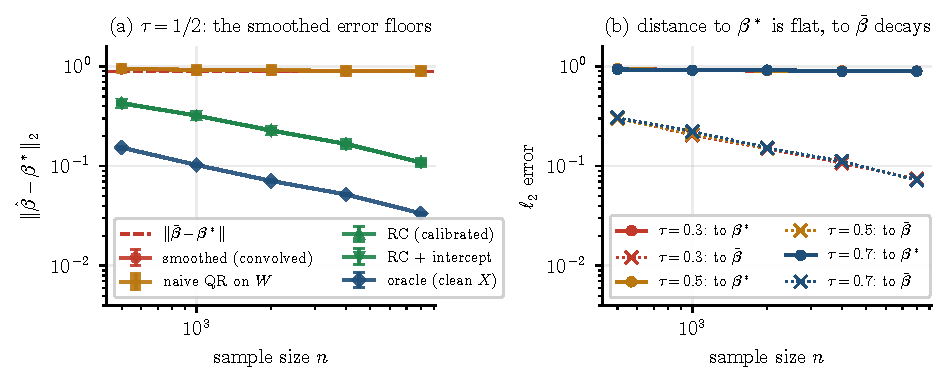
\includegraphics[width=0.95\textwidth]{../figures/fig2_scaling.pdf}
    \caption{$\ell_2$ error as a function of $n$ ($p=10$, $s=5$,
    $\sigma_u=0.5$, $50$ replications, unpenalised). Panel (a), at $\tau=1/2$: the smoothed
    estimator (``convolved'') is flat and sits at the attenuation floor
    $\norm{\bbar-\betas}$ (dashed line); the calibrated estimator (``RC$+$int'') has the
    oracle's $\sqrt n$ slope, offset by the efficiency factor of
    Remark~\ref{rem:efficiency}. Panel (b): the same smoothed estimates measured instead
    against $\bbar$, for the three quantile levels; the solid curves, which are distances to
    $\betas$, do not decay, while the dotted curves, which are distances to $\bbar$,
    decrease at the $\sqrt n$ rate. The three levels coincide to within Monte-Carlo error,
    as the $\tau$-independence of $\bbar$ requires.}
    \label{fig:scaling}
\end{figure}

\subsection{High dimensions}
\label{sec:highdim-sim}

Table~\ref{tab:highdim} and Figure~\ref{fig:highdim} report the high-dimensional
comparison at $n=400$, $p=500$, $s=10$, $\tau=1/2$, $\lambda=0.02$, with $30$
replications and a fixed $\betas$. The smoothed two-stage estimator follows the published
algorithm of that method, reimplemented in the code accompanying this paper; naive,
calibrated and oracle
estimators are fitted with an exact
linear-programming solver, so no difference can be attributed to optimisation error.

In \emph{total} $\ell_2$ error the smoothed estimator is competitive, and at
$\sigma_u=0.1$ it matches the oracle ($0.73$ versus $0.75$), because at this $(n,p)$ the
error is dominated by variance and the smoothed objective, with its pilot scale, is
strongly convex and hence low-variance. This is a genuine bias--variance trade-off, and it
is why such estimators look attractive in small samples. The trade-off, however, is with a
bias that never disappears. The probability limit of the
smoothed estimator is $\bbar$, at distance $\norm{\bbar-\betas} = 0.06$, $0.52$ and $1.25$
from $\betas$ at $\sigma_u=0.1,0.3,0.5$; its realised distance to $\bbar$ in this
experiment is $0.71$, $1.09$ and $1.53$, i.e.\ the bias is buried under estimation noise
at $n=400$. Table~\ref{tab:scaling} shows what happens when the noise is reduced, and no
amount of additional data removes the bias. The calibrated estimator is unbiased here as
well, but visibly less efficient than
the oracle: median $1.51$ versus $0.75$ at $\sigma_u=0.3$ and $2.10$ versus $0.75$ at
$\sigma_u=0.5$, in line with the variance inflation predicted in
Remark~\ref{rem:efficiency}. The convolution $e_i = V_i^\top\betas+\varepsilon_i$ flattens the
error density at the quantile, and the calibrated regressor is attenuated. At
this $(n,p)$ the biased smoothed estimator therefore has the smaller total error at all three
measurement-error levels ($0.73$/$1.24$/$1.83$ versus $0.88$/$1.51$/$2.10$).
Table~\ref{tab:highdim} is a statement about efficiency in a variance-dominated
regime, not evidence that the smoothed estimator identifies $\betas$, and this is the
regime in which a bias floor is hardest to detect by simulation.

\begin{table}[ht]
\centering
\footnotesize
\setlength{\tabcolsep}{3pt}
\caption{High-dimensional comparison ($n=400$, $p=500$, $s=10$, $\tau=1/2$, $\lambda=0.02$, $R=30$, fixed $\betas$): median $\ell_2$ error against $\betas$, IQR in parentheses. ``smoothed'' is the two-stage smoothed estimator, following the published algorithm of that method as reimplemented in the code accompanying this paper; ``naive'', ``RC'' and ``oracle'' are exact linear-programming quantile regressions on $W$, on the calibrated $\muv=\Ccal W$, and on the clean $X$. The error is variance-dominated here, so the smoothed estimator is competitive in $\ell_2$ although it targets $\bbar$; its distance to $\bbar$, reported beneath each block, stays bounded away from zero.}
\label{tab:highdim}
\begin{tabular}{lcccc}
\toprule
$\sigma_u$ & smoothed & naive & RC & oracle \\
\midrule
0.1 & 0.734 (0.703, 0.789) & 0.892 (0.863, 0.960) & 0.878 (0.848, 0.944) & 0.746 (0.734, 0.779) \\
\multicolumn{5}{l}{\quad smoothed: $\norm{\bbar-\betas}_2=0.062$, $\norm{\hat\beta-\bbar}_2=0.713$} \\
\midrule
0.3 & 1.236 (1.172, 1.354) & 1.639 (1.551, 1.746) & 1.514 (1.443, 1.592) & 0.746 (0.734, 0.779) \\
\multicolumn{5}{l}{\quad smoothed: $\norm{\bbar-\betas}_2=0.517$, $\norm{\hat\beta-\bbar}_2=1.088$} \\
\midrule
0.5 & 1.830 (1.731, 1.933) & 2.493 (2.384, 2.645) & 2.097 (2.025, 2.153) & 0.746 (0.734, 0.779) \\
\multicolumn{5}{l}{\quad smoothed: $\norm{\bbar-\betas}_2=1.253$, $\norm{\hat\beta-\bbar}_2=1.530$} \\
\bottomrule
\end{tabular}
\end{table}


\begin{figure}[ht]
    \centering
    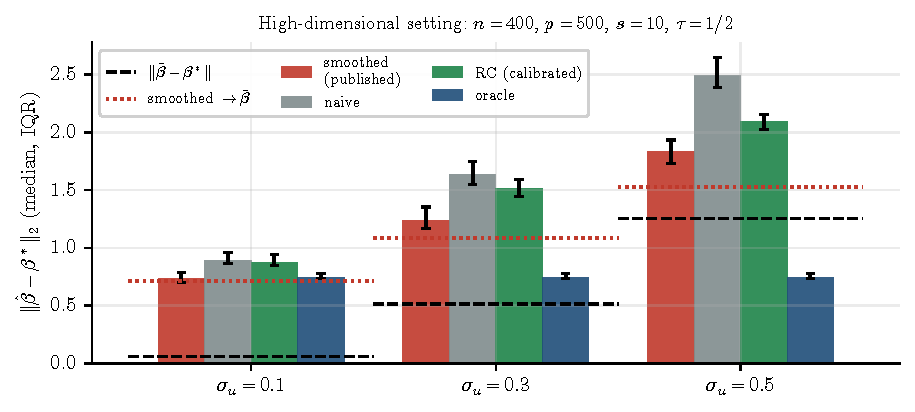
\includegraphics[width=0.95\textwidth]{../figures/fig3_highdim.pdf}
    \caption{High-dimensional comparison ($n=400$, $p=500$, $s=10$, $\tau=1/2$, $30$
    replications; medians with interquartile ranges). The smoothed estimator is
    competitive in total $\ell_2$ error in this variance-dominated regime, but its
    probability limit is the attenuation target $\bbar$ (dashed line), so its distance to
    $\betas$ is bounded below by the floor $\norm{\bbar-\betas}$, which no sample size
    removes; its realised distance to $\bbar$ (dotted line) is $0.71$, $1.09$ and $1.53$ at
    $\sigma_u=0.1,0.3,0.5$ here, so at this sample size the bias is buried under estimation
    noise and Table~\ref{tab:scaling} is what reveals it. The calibrated estimator is
    unbiased for $\betas$ and has the oracle's convergence rate
    (Table~\ref{tab:scaling}).}
    \label{fig:highdim}
\end{figure}

\subsection{Inference}
\label{sec:coverage}

Theorem~\ref{thm:lowdim} asserts that the calibrated estimator is asymptotically normal
with the usual quantile-regression sandwich covariance. Table~\ref{tab:coverage} verifies
this directly, and at the same time makes the cost of the target shift concrete. Wald
intervals for the calibrated estimator cover $\betas$ at $0.89$--$0.93$ (nominal $90\%$)
and $0.93$--$0.97$ (nominal $95\%$) across $n$ and $\tau$. Intervals built from the
smoothed score, using its own correct sandwich covariance, are equally well calibrated, at
$0.93$--$0.97$ for a nominal $95\%$, but for $\bbar$: their coverage of $\betas$
is $0.000$ in all twelve cells, i.e.\ not a single one of the $4{,}800$ smoothed intervals
contained the true coefficient when $\sigma_u=0.5$. This is the operational form of
Theorem~\ref{thm:score}: the smoothing does not destroy the calibration of the interval, it
changes the parameter the interval is about. It also explains why no resampling scheme can
repair inference for the smoothed estimator (Remark~\ref{rem:subsampling}): the problem is not the width of the interval but its centre.

\begin{table}[ht]
\centering
\small
\caption{Coverage of nominal $90\%$ and $95\%$ Wald intervals ($\sigma_u=0.5$, $\betas=2$, $\bbar=1.6$, 400 replications). Intervals use the sandwich covariance of Theorem~\ref{thm:lowdim} for the calibrated estimator and the corresponding smoothed-score covariance for the smoothed estimator. The calibrated intervals cover $\betas$ at close to the nominal rate; the smoothed intervals are equally well calibrated, but for $\bbar$, and cover $\betas$ essentially never.}
\label{tab:coverage}
\begin{tabular}{cccccc}
\toprule
& & \multicolumn{2}{c}{calibrated, target $\betas$} & \multicolumn{2}{c}{smoothed, $95\%$} \\
$\tau$ & $n$ & $90\%$ & $95\%$ & covers $\betas$ & covers $\bbar$ \\
\midrule
0.3 & 500 & 0.920 & 0.953 & 0.000 & 0.958 \\
0.3 & 1000 & 0.902 & 0.943 & 0.000 & 0.955 \\
0.3 & 2000 & 0.897 & 0.932 & 0.000 & 0.940 \\
0.3 & 4000 & 0.892 & 0.948 & 0.000 & 0.948 \\
0.5 & 500 & 0.890 & 0.945 & 0.000 & 0.945 \\
0.5 & 1000 & 0.902 & 0.970 & 0.000 & 0.953 \\
0.5 & 2000 & 0.912 & 0.950 & 0.000 & 0.925 \\
0.5 & 4000 & 0.925 & 0.968 & 0.000 & 0.968 \\
0.7 & 500 & 0.897 & 0.945 & 0.000 & 0.950 \\
0.7 & 1000 & 0.932 & 0.973 & 0.000 & 0.955 \\
0.7 & 2000 & 0.920 & 0.963 & 0.000 & 0.945 \\
0.7 & 4000 & 0.912 & 0.960 & 0.000 & 0.945 \\
\bottomrule
\end{tabular}
\end{table}


\begin{remark}[The naive score, checked]
Corollary~\ref{cor:same-target} can be checked on the same data. At $\sigma_u=0.5$ the
Monte-Carlo estimate of $\E[W_i(\tau-\ind{r_i^*<0})]$ is $-0.13086\,(\pm0.00086)$ for
$\tau=1/2$, against the analytic value $-0.13079$ from \eqref{eq:naive-bias}, which is
$-\norm{\Sigma_u\betas}_1d_{\mathrm{naive}}$ with
$d_{\mathrm{naive}}=(\cN(0,\sigma^{*2})*f_\varepsilon)(0)=0.2616$; for
$\tau=0.3$ and $0.7$ the estimates are $-0.16105$ and $-0.16156$ against $-0.16166$ and
$-0.16169$, i.e.\ $d_{\mathrm{naive}}=0.3234$ for the asymmetric Laplace law used at those
levels. The two constants differ because the error laws differ in scale, not in shape: at
$\tau=1/2$ we generate Laplace$(0,1)$, whose density at the quantile is $1/2$, whereas for
$\tau\neq1/2$ we generate $\varepsilon=(1-\tau)E_1-\tau E_2$ with $E_j\sim\mathrm{Exp}(1)$,
whose density at the quantile is $1$. All other quantities reported below are free of that
scale. The naive and the smoothed score are therefore biased by the same mechanism
and to the same order, which is why their population targets coincide
(Table~\ref{tab:targets}).
\end{remark}

\subsection{Estimated calibration in high dimensions}
\label{sec:hd-est}

Table~\ref{tab:hdc} tests the chain of \S\ref{sec:estimated} in a design where the
plug-in is least favourable on paper: $\Sigma_x$ is banded Toeplitz with row sparsity
$11$, so $\Ccal=\Sigma_x(\Sigma_x+\Sigma_u)^{-1}$ is \emph{dense}, and $\hat\Sigma_x$ is
obtained by Ledoit--Wolf shrinkage followed by entrywise hard thresholding.

The calibration matrix is estimated accurately: $\|\hat\Ccal-\Ccal\|_2$ is
$0.005$, $0.039$ and $0.088$ at $\sigma_u=0.1,0.3,0.5$, one to two orders of
magnitude below the scale of the coefficients. Consequently the plug-in
estimator is statistically indistinguishable from the oracle-calibration estimator
(differences of at most $0.02$ in $\ell_2$ error, within one standard error at every
$\sigma_u$), while both improve substantially on the naive estimator once the
attenuation matters: at $\sigma_u=0.5$, $1.564$ versus $1.808$ with the oracle at $1.545$.
The sup-norm score is the quantity the proof turns on, and estimating the
calibration does not inflate it: $\|n^{-1}\sum_i{\hat{\muv}}_i\psi_i\|_\infty$ equals
$0.0831$, $0.0793$, $0.0732$ against $0.0832$, $0.0793$, $0.0734$ for the oracle design,
all below the theoretical scale $\sqrt{\log p/n}=0.1246$. The nodewise inverse is exact on
the reported coordinates, $\max_j|(\hat\Theta\hat H)_{jj}-1|=0$ to machine precision. In this
design, therefore, the
sufficient condition of Assumption~\ref{ass:calib-acc} is satisfied with room to spare,
even though Lemma~\ref{lem:perturb} alone would only certify the spectral norm.

Theorem~\ref{thm:estimated} is conditional on
row-wise accuracy of $\hat\Ccal$; we have not proved that thresholding delivers it for
growing row sparsity, and Remark~\ref{rem:spectral-not-enough} explains why the spectral
norm alone cannot be enough. What Table~\ref{tab:hdc} shows is that the gap between the
provable condition and what the plug-in actually needs is not vacuous in the
banded-$\Sigma_x$ designs that arise in practice, and it identifies the quantity that a
sharper theory, or a bias-corrected design, would have to control: the sup-norm score.

\begin{table}[ht]
\centering
\footnotesize
\setlength{\tabcolsep}{3pt}
\caption{Estimated calibration in high dimensions ($n=400$, $p=500$, $s=10$, $\tau=0.5$, $R=30$ replications, banded $\Sigma_x$, $\hat\Sigma_x$ from thresholded Ledoit--Wolf shrinkage). $\hat\Ccal$ is computed from the estimated $\hat\Sigma_x$; the oracle column uses the true $\Ccal$. The sup-norm scores are evaluated at the truth, $\|n^{-1}\sum_i{\hat\muv}_i\psi_i\|_\infty$, with the theoretical scale $\sqrt{\log p/n} = 0.1246$.}
\label{tab:hdc}
\begin{tabular}{lccccc}
\toprule
$\sigma_u$ & $\|\hat\Ccal-\Ccal\|_2$ & naive & oracle $\Ccal$ & estimated $\hat\Ccal$ & sup-norm score (oracle / estimated) \\
\midrule
0.1 & 0.0051 & 0.822 & 0.816 & 0.815 & 0.0832 / 0.0831 \\
0.3 & 0.0393 & 1.269 & 1.183 & 1.184 & 0.0793 / 0.0792 \\
0.5 & 0.0882 & 1.808 & 1.545 & 1.564 & 0.0734 / 0.0732 \\
\bottomrule
\end{tabular}
\end{table}


\subsection{Efficiency of the calibrated estimator}
\label{sec:efficiency}

Remark~\ref{rem:efficiency} quantified the price of measurement error as
an efficiency loss: $f_e(\delta_\tau)<f_\varepsilon(0)$ because $e_i$ convolves
$\varepsilon_i$ with $V_i^\top\betas$, and the calibrated regressor is attenuated. It is
natural to ask whether that loss can be bought back. One route is available in principle
and cheap: in the location-shift model every quantile level estimates the same $\betas$, so
the estimators $\hat\beta_{\tau_1},\dots,\hat\beta_{\tau_K}$ can be combined. Their joint
asymptotic covariance is, in units of $\E[\muv\muv^\top]^{-1}$,
\begin{equation}
C_{kl} = \frac{\tau_k\wedge\tau_l-\tau_k\tau_l}{f_kf_l},
\qquad f_k = f_e\big(Q_{\tau_k}(e)\big),
\label{eq:gls}
\end{equation}
so the GLS combination has variance $(1^\top C^{-1}1)^{-1}$ against $C_{\tau_0\tau_0}$ for
the single level $\tau_0$. Table~\ref{tab:gls} evaluates the ratio. For Laplace errors it
is exactly $1$: the median is already the most efficient quantile and combining adds
nothing. For Gaussian and uniform errors the gain is real, up to a $30\%$ reduction in
variance (a $16\%$ reduction in standard error) with seven levels.

\begin{table}[ht]
\centering
\small
\caption{Theoretical gain from combining quantile levels in the location-shift model: ratio of the GLS variance \eqref{eq:gls} to the variance of the single level $\tau=1/2$, computed from the closed form. The levels combined are $\{0.40,0.50,0.60\}$ (3), $\{0.35,0.40,\dots,0.65\}$ in steps of $0.05$ (7) and $\{0.1,0.2,\dots,0.9\}$ (9), each set containing $\tau=1/2$. A value of $1$ means combining levels recovers nothing.}
\label{tab:gls}
\begin{tabular}{lccc}
\toprule
error distribution & 3 levels & 7 levels & 9 levels \\
\midrule
Laplace & 1.0000 & 1.0000 & 1.0000 \\
Gaussian & 0.8494 & 0.7977 & 0.6638 \\
Uniform & 0.8000 & 0.7000 & 0.2000 \\
\bottomrule
\end{tabular}
\end{table}


Two conclusions. First, the part of the efficiency loss caused by the flattened density
$f_e$ is \emph{not} recoverable by reweighting quantile moments: all of them share the same
$f_e$, so the loss appears in every $C_{kk}$ and cancels in the ratio
\eqref{eq:gls}. Second, what is recoverable is the part caused by looking at a single
quantile of an error distribution whose density is not concentrated there, and the
recovery is free of any modelling beyond the location-shift structure. A simulation with
$K=7$ levels and weights estimated by kernel density confirms the direction for Gaussian
errors (ratio $0.90$ at $n=1000$, against an asymptotic optimum of $0.80$ that requires
accurate weights); for Laplace errors the same implementation returned $0.91$, which the
theory says cannot be a genuine gain, since the oracle design moved in the opposite
direction; we therefore report it as an artefact of estimated weights rather than an
improvement. The remaining route to efficiency is to use more information than
$(Y,\muv)$: conditioning on $(Y,W)$ rather than $W$ alone, as in the conditional
estimating equations of \citet{wei2009quantile}, does that, at the cost of
modelling the quantile process. Carrying that construction into $p\gg n$ is open.

\subsection{Population targets of the estimators fitted on the raw $W$}
\label{sec:targets-si}

Table~\ref{tab:targets} reports the exact population targets plotted in Figure~\ref{fig:loss},
for $p=1$ and $N=2\times10^5$: the minimiser of each population objective, computed without an
optimiser (subgradient root-finding for the check loss, grid search with parabolic refinement
for the smoothed loss).

\begin{table}[ht]
\centering
\footnotesize
\caption{Exact population targets of the estimators fitted on the raw $W$ (scalar case, $X\sim\cN(0,1)$, $N=2\times10^5$; each entry is the minimiser of a population objective, computed without an optimiser). $\betas=2$; $\bbar=\Sigma_x(\Sigma_x+\Sigma_u)^{-1}\betas$ is the attenuation target. By Proposition~\ref{prop:exact-target} the population minimiser is exactly $\bbar$ for naive quantile regression and for every fixed-scale smoothed loss, and exactly $(\Sigma_x+\Sigma_u+M)^{-1}\Sigma_x\betas$ for the adaptive scale with kernel $M$; the tabulated Monte-Carlo values agree with those exact values to within $0.006$, the largest deviation over the table (the posterior-kernel column is within $0.004$ of $\bbar$ (Proposition~\ref{prop:posterior-adaptive}). Column 5 uses the pilot scale $\sigmah$ from a calibrated Stage~1 (idealised: the true $\Sigma_x$ is used, which favours the smoothed method).}
\label{tab:targets}
\begin{tabular}{llcccccc}
\toprule
$\sigma_u$ & $\tau$ & $\bbar$ & smoothed & smoothed & smoothed & smoothed & naive \\
 & & & (fixed $\sigma$) & (pilot $\sigmah$) & (adaptive) & (post.\ kernel) & \\
\midrule
0.1 & 0.3 & 1.980 & 1.979 & 1.979 & 1.960 & 1.979 & 1.978 \\
0.1 & 0.5 & 1.980 & 1.982 & 1.982 & 1.963 & 1.982 & 1.982 \\
0.1 & 0.7 & 1.980 & 1.979 & 1.979 & 1.960 & 1.980 & 1.979 \\
\midrule
0.3 & 0.3 & 1.835 & 1.831 & 1.831 & 1.692 & 1.832 & 1.832 \\
0.3 & 0.5 & 1.835 & 1.840 & 1.840 & 1.699 & 1.839 & 1.840 \\
0.3 & 0.7 & 1.835 & 1.834 & 1.834 & 1.693 & 1.832 & 1.834 \\
\midrule
0.5 & 0.3 & 1.600 & 1.599 & 1.599 & 1.333 & 1.599 & 1.600 \\
0.5 & 0.5 & 1.600 & 1.600 & 1.599 & 1.333 & 1.599 & 1.597 \\
0.5 & 0.7 & 1.600 & 1.601 & 1.601 & 1.334 & 1.600 & 1.602 \\
\bottomrule
\end{tabular}
\end{table}


\subsection{Real data: dietary intake and body mass index}
\label{sec:nhanes-si}

Here the measurement-error covariance is estimated from replicates.
NHANES 2017--2018 records two 24-hour dietary recalls for each participant, so the same
quantity is measured twice, and under the classical model the pair identifies both
\begin{equation}
\Sigma_x = \mathrm{Cov}(R_1,R_2),
\qquad
\Sigma_u = \tfrac12\,\mathrm{Var}(R_1-R_2),
\label{eq:replicates}
\end{equation}
with no assumption on $\Sigma_u$ beyond the model itself. We take the $24$ nutrient totals
reported in both recalls, body mass index as the response, and adults aged $20+$ with two
reliable recalls and complete records ($n=3649$).

The nutrients are strongly collinear (total fat and monounsaturated fat correlate at
$0.97$, total fat and saturated fat at $0.93$, protein and phosphorus at $0.90$), so
$\hat\Sigma_x$ has condition number $2\times10^4$ and $\hat\Ccal$ is numerically explosive,
the ill-conditioning that \S\ref{sec:estimated} warns about. We remove the near-duplicates
(total, mono- and poly-unsaturated fat; phosphorus; potassium; moisture), leaving $p=18$
nutrients with $\mathrm{cond}(\hat\Sigma_x+\Sigma_u)
= 585$. Regularising $\hat\Sigma_x$ instead (banding or thresholding \citep{bickel2008},
linear shrinkage \citep{ledoit2004}) would control the conditioning but change $\hat\Ccal$
and hence the target, so we prune rather than estimate a different calibration. The
estimated reliabilities $(\hat\Sigma_x)_{jj}/((\hat\Sigma_x)_{jj}+(\hat\Sigma_u)_{jj})$
average $0.417$: a single 24-hour recall carries more measurement variance than signal.

Table~\ref{tab:nhanes} reports the results. The naive coefficients are attenuated by
roughly a factor of six, the median ratio of naive to calibrated coefficients being
$0.156$; collinearity makes the attenuation \emph{worse} than the mean reliability of
$0.417$ would suggest for a single covariate. The correction
changes magnitudes (energy: $3.2$ to $22.7$; carbohydrate: $-1.7$ to $-12.3$) and
conclusions: ten of the eighteen coefficients have debiased intervals excluding zero,
against nine for the naive analysis at the same level, but the sets are not nested. The
intervals are wide: saturated fat moves from $-0.65$ to $-6.21$, its interval
$[-11.7,0.7]$ still containing zero, so the correction enlarges the estimate without
establishing it.

This is an illustration, not a validation. The truth is unknown, so nothing here checks
accuracy; the outcome is itself measured with error; the two recalls are not independent
draws, so \eqref{eq:replicates} is at best a working
approximation, and our $\hat\Sigma_x$ does have one slightly negative eigenvalue; survey
weights are not used; and the near-duplicates had to be removed before the
calibration could be computed at all.

\begin{table}[ht]
\centering
\footnotesize
\setlength{\tabcolsep}{4pt}
\caption{Real data: NHANES 2017--2018, $n=3649$ adults with two reliable 24-hour dietary recalls, $p=18$ nutrients after removing near-duplicates, $\tau=1/2$. Both $\Sigma_x$ and $\Sigma_u$ are estimated from the replicate pair, with no synthetic noise; reliability is $(\Sigma_x)_{jj}/((\Sigma_x)_{jj}+(\Sigma_u)_{jj})$. ``naive'' uses the day-1 recall and ``calibrated'' uses $\hat\Ccal W$ with an intercept and the debiased interval of \S\ref{sec:debiasing}; the largest $10$ coefficients in absolute value are shown.}
\label{tab:nhanes}
\begin{tabular}{lcccr}
\toprule
nutrient & reliability & naive & calibrated & $95\%$ interval \\
\midrule
energy & 0.449 & +3.200 & +22.749 & $[+7.18,\, +34.70]$$^{\dagger}$ \\
protein & 0.397 & +1.250 & +14.657 & $[+3.03,\, +26.30]$$^{\dagger}$ \\
zinc & 0.394 & -2.051 & -13.589 & $[-20.46,\, -4.63]$$^{\dagger}$ \\
carbohydrate & 0.462 & -1.680 & -12.253 & $[-23.27,\, -0.90]$$^{\dagger}$ \\
magnesium & 0.486 & -2.139 & -10.283 & $[-15.95,\, -4.28]$$^{\dagger}$ \\
calcium & 0.394 & +1.386 & +8.579 & $[+4.14,\, +11.95]$$^{\dagger}$ \\
iron & 0.393 & +1.610 & +6.814 & $[+0.74,\, +12.70]$$^{\dagger}$ \\
saturated fat & 0.398 & -0.651 & -6.206 & $[-11.74,\, +0.71]$ \\
folate & 0.360 & -1.484 & -5.697 & $[-10.80,\, -1.16]$$^{\dagger}$ \\
vitamin D & 0.318 & -1.066 & -2.837 & $[-5.54,\, +0.24]$ \\
\midrule
\multicolumn{5}{l}{$^{\dagger}$interval excludes zero.}\\
\bottomrule
\end{tabular}
\end{table}


\section{Reproducibility}
\label{app:repro}

\sloppy
\texttt{simulations/routeA\_\allowbreak lib.py} holds the solvers (damped Newton for the smoothed loss and
Frobenius-norm helpers) and the data generators; \texttt{routeA\_\allowbreak targets.py} computes the exact
population targets of Table~\ref{tab:targets}, computed without any optimiser
(subgradient root-finding, profiling, grid search).

\texttt{routeA\_\allowbreak experiments.py}: the score check, the scaling study and the
high-dimensional comparison (Tables~\ref{tab:score}--\ref{tab:highdim});
\texttt{routeA\_\allowbreak inference.py}: the coverage study of Table~\ref{tab:coverage} and the
naive-score check.

\texttt{hdc\_\allowbreak experiments.py}: estimated calibration in high dimensions
(Table~\ref{tab:hdc}); \texttt{hdc\_\allowbreak gls\_\allowbreak theory.py}: the closed-form GLS gains of
Table~\ref{tab:gls}.

\texttt{hdc\_\allowbreak debias\_\allowbreak final.py} ($p<n$) and \texttt{hdc\_\allowbreak pgtn.py} ($p>n$, nodewise
inverse) produce the debiasing study of Table~\ref{tab:debias};
\texttt{hdc\_\allowbreak debias\_\allowbreak diag.py} and \texttt{hdc\_\allowbreak debias\_\allowbreak fix.py} contain the diagnostics that
identified the $\ell_1$ initial bias as the cause of the pilot failure.

\texttt{routeA\_\allowbreak tables.py} and \texttt{routeA\_\allowbreak figures.py}: generate every table
and figure of this paper directly from the saved JSON results, so that the numbers in the
text cannot drift from the code. The population curves of Figure~\ref{fig:loss} are
evaluated by Gauss-Laguerre quadrature in the Laplace error density, using the Gaussian
reduction of \eqref{eq:cal-gauss}, and their minimisers are located by one-dimensional
bounded optimisation of the quadrature, so no simulation error enters that figure.

\texttt{nhanes\_\allowbreak realdata.py}: the application of \S\ref{sec:nhanes}: merges the
four NHANES public-use files, estimates $\Sigma_x$ and $\Sigma_u$ from the two dietary
recalls, prunes near-duplicate nutrients, and fits the naive, calibrated and debiased
estimators (Table~\ref{tab:nhanes}).

\texttt{consistency\_\allowbreak audit.py}: re-derives every number typed by hand in the text
from the JSON results and the closed-form expressions, and checks it against the
manuscript; it covers all tables, the Monte-Carlo verification of
Theorem~\ref{thm:adaptive}, the numerical claims attached to
Proposition~\ref{prop:posterior-adaptive}, and the real-data numbers of
\S\ref{sec:nhanes}.

\texttt{review/}: the independent checks of the smoothed loss's target
(\texttt{verify\_\allowbreak corrected\_\allowbreak target.py}), of the calibration repair
(\texttt{verify\_\allowbreak rc\_\allowbreak fix.py}), of Proposition~\ref{prop:posterior-adaptive}
(\texttt{verify\_\allowbreak posterior\_\allowbreak adaptive.py}, which verifies the Gaussian reduction
\eqref{eq:cal-gauss}, the monotonicity in $\varsigma$ and the location of the minimiser in
nine scalar cells and in a matrix case where $\Sigma_x$ and $\Sigma_u$ do not commute), of
the quadrature used for Figure~\ref{fig:loss} against a direct simulation of the model
(\texttt{verify\_\allowbreak fig1\_\allowbreak exact\_\allowbreak curves.py}), of the determinism of the debiasing study
(\texttt{verify\_\allowbreak debias\_\allowbreak determinism.py}), and the reference audit
(\texttt{reference\_\allowbreak audit.md}).
\fussy

\section*{Code and data availability}
\addcontentsline{toc}{section}{Code and data availability}

All numerical results in this paper are produced by the scripts listed in
Appendix~\ref{app:repro}, which are self-contained Python files. Each table and figure is
generated directly from the saved JSON output of those scripts, so the numbers reported
here cannot drift from the code that produced them. The scripts, their saved output and the
independent verification scripts are archived in a version-controlled repository and on
Zenodo, at \url{https://doi.org/10.5281/zenodo.23175827} (repository:
\url{https://github.com/CIKIXI/smoothed-check-loss-trap}). All data are publicly available: the
simulation designs use synthetic Gaussian covariates and known Gaussian measurement error,
so they need no external data, and the application in \S\ref{sec:nhanes} uses the NHANES
2017--2018 public-use demographic, body-measure and two 24-hour dietary-recall files. No
other data set is used, and in the application the measurement-error covariance is
estimated from the two dietary recalls rather than assumed. The public-use files are
archived by the US Centers for Disease Control and Prevention at
\begin{center}
\texttt{https://wwwn.cdc.gov/nchs/nhanes/}
\end{center}

\section*{Acknowledgments and funding}
\addcontentsline{toc}{section}{Acknowledgments and funding}

The author gratefully acknowledges the developers of the NumPy, SciPy and scikit-learn
packages, which were used for all computations reported here, and the US Centers for
Disease Control and Prevention for making the NHANES public-use data available. The author
declares no conflicts of interest. This work was not supported by any funding agency.

\clearpage
\bibliographystyle{plainnat}
\bibliography{references}

\end{document}
